% ---------- Titelblad Masterproef Faculteit Wetenschappen -----------
% Dit document is opgesteld voor compilatie met pdflatex.  Indien je
% wilt compileren met latex naar dvi/ps, dien je de figuren naar
% (e)ps-formaat om te zetten.
%                           -- december 2012
% -------------------------------------------------------------------
\RequirePackage{fix-cm}
\documentclass[12pt,a4paper,oneside]{book}

% --------------------- In te laden pakketten -----------------------
% Deze kan je eventueel toevoegen aan de pakketten die je al inlaadt
% als je dit titelblad integreert met de rest van thesis.
% -------------------------------------------------------------------
\usepackage{graphicx,xcolor,textpos}
\usepackage{helvet}
\usepackage{tikz}
\usetikzlibrary{fit,shapes,arrows,positioning,calc}
\usepackage{wrapfig}
\usepackage{chngcntr}
\usepackage{amsmath}
\usepackage{amssymb}
\usepackage{graphicx,caption}
\usepackage{subcaption}
\usepackage[utf8]{inputenc}
\usepackage{soul}
\usepackage{multirow}
\usepackage{afterpage}
\usepackage{array}
\usepackage{ragged2e}
\usepackage{enumitem}

\newcommand\blankpage{%
    \null
    \thispagestyle{empty}%
    \addtocounter{page}{-1}%
    \newpage}
    
\counterwithout{figure}{chapter}
\counterwithout{table}{chapter}
\newcommand\tab[1][1cm]{\hspace*{#1}}
\usepackage[ruled]{algorithm2e}
\makeatletter
\renewcommand{\algorithmcfname}{Algoritme}
\newcommand{\RemoveAlgoNumber}{\renewcommand{\fnum@algocf}{\AlCapSty{\AlCapFnt\algorithmcfname}}}
\newcommand{\RevertAlgoNumber}{\algocf@resetfnum}
\makeatother

\usepackage[acronym]{glossaries}
\newacronym{fcc}{FCC}{Freely Chosen Cadence}
\newacronym{cvt}{CVT}{Continu Variabele Transmissie}
\newacronym{dt}{DT}{Decision Tree}
\newacronym{pa}{PA}{Passive Aggressive}
\newacronym{rf}{RF}{Random Forest}
\newacronym{ma}{MA}{Moving \ Average \ }
\newacronym{es}{ES}{Exponential \ Smoothing \ }
\newacronym{mse}{MSE}{Mean Squared Error}
\newacronym{dc}{DC}{Direct Current}
\newacronym{dea}{DEA}{Droplet Ensemble Algorithm}

\newglossaryentry{delta_c}{
  name = \ensuremath{\Delta_c} ,
  description = Absoluut verschil tussen fietsersmodel en voorspelling,
}
\newglossaryentry{lambda}{
  name = \ensuremath{\lambda} ,
  description = Applicatie specifieke parameter van biased reservoir sampling,
}
\newglossaryentry{r}{
  name = \ensuremath{r} ,
  description = Input vector fietser,
}
\newglossaryentry{u_cy}{
  name = \ensuremath{u_{cy}} ,
  description = Input vector fiets\,{} geleverd door de fietser,
}
\newglossaryentry{u_contr}{
  name = \ensuremath{u_{contr}} ,
  description = Input vector fietser\,{} geleverd door de controller
}
\newglossaryentry{y}{
  name = \ensuremath{y} ,
  description = Output vector fiets
}
\newglossaryentry{fcc_est}{
  name = \ensuremath{FCC_{est}} ,
  description = Schatting van FCC\,{} geleverd door de cadanscontroller,
}
\newglossaryentry{v_ref}{
  name = \ensuremath{v_{ref}} ,
  description = Referentie snelheid van de fietser,
}
\newglossaryentry{t_cy}{
  name = \ensuremath{T_{cy}} ,
  description = Koppel geleverd door de fietser,
}
\newglossaryentry{t_cy,m}{
  name = \ensuremath{T_{cy,m}} ,
  description = Gemeten koppel geleverd door de fietser,
}
\newglossaryentry{u_c}{
  name = \ensuremath{u_c} ,
  description = Toestands variabele die bepaalt of de cadans moet veranderen,
}
\newglossaryentry{theta_cr}{
  name = \ensuremath{\theta_{cr}} ,
  description = Hoek van de trapas,
}
\newglossaryentry{v_bike}{
  name = \ensuremath{v_{bike}} ,
  description = Snelheid van de fiets,
}
\newglossaryentry{helling}{
  name = \ensuremath{\alpha} ,
  description = Helling,
}
\newglossaryentry{t_dc}{
  name = \ensuremath{T_{dc}} ,
  description = Het DC-koppel van de fietser (gemiddeld koppel),
}
\newglossaryentry{t_dc_max}{
  name = \ensuremath{T_{dc,max}} ,
  description = Maximum DC-koppel dat geleverd kan worden,
}
\newglossaryentry{omega_cr}{
  name = \ensuremath{\omega_{cr}} ,
  description = Cadans in rpm,
}
\newglossaryentry{fcc_pred}{
  name = \ensuremath{FCC_{pred}},
  description = Voorspelde FCC,
}
\newglossaryentry{k_cr,r}{
  name = \ensuremath{k_{cr,r}} ,
  description = Verhouding overbrenging trapas-ringwiel,
}
\newglossaryentry{nr}{
  name = \ensuremath{nr} ,
  description = Aantal tanden op het ringwiel,
}
\newglossaryentry{ns}{
  name = \ensuremath{ns} ,
  description = Aantal tanden op het zonnewiel,
}
\newglossaryentry{s}{
  name = \ensuremath{S} ,
  description = Ondersteuningsniveau,
}
\newglossaryentry{f_grav}{
  name = \ensuremath{F_{grav}} ,
  description = Gravitationele last,
}
\newglossaryentry{f_friction}{
  name = \ensuremath{F_{friction}} ,
  description = Wrijvings last,
}
\newglossaryentry{f_aero}{
  name = \ensuremath{F_{aero}} ,
  description = Luchtweerstand,
}
\newglossaryentry{f_load}{
  name = \ensuremath{F_{load}} ,
  description = Totale last,
}
\newglossaryentry{m}{
  name = \ensuremath{m} ,
  description = Totaal gewicht van fiets en fietser,
}
\newglossaryentry{g}{
  name = \ensuremath{g} ,
  description = Gravitationele constante,
}
\newglossaryentry{c_r}{
  name = \ensuremath{c_r} ,
  description = Rolweerstand coëfficiënt,
}
\newglossaryentry{c_d}{
  name = \ensuremath{c_d} ,
  description = Luchtweerstand coëfficiënt,
}
\newglossaryentry{rho_aero}{
  name = \ensuremath{\rho_{aero}} ,
  description = Luchtdichtheid,
}
\newglossaryentry{a_aero}{
  name = \ensuremath{A_{aero}} ,
  description = Frontaal oppervlak fietser,
}
\newglossaryentry{t_mg2}{
  name = \ensuremath{T_{MG2}} ,
  description = Koppel geleverd door motor op het voorwiel,
}
\newglossaryentry{t_rw}{
  name = \ensuremath{T_{rw}} ,
  description = Koppel op het achterwiel,
}
\newglossaryentry{r_w}{
  name = \ensuremath{r_w} ,
  description = Straal van het voor- en achterwiel,
}
\newglossaryentry{p}{
  name = \ensuremath{P} ,
  description = Vermogen,
}
\newglossaryentry{sf}{
  name = \ensuremath{sf} ,
  description = Smoothing factor,
}
\newglossaryentry{f_k}{
  name = \ensuremath{f_k} ,
  description = Factor voor fietsersmodel in functie van het gemiddeld koppel,
}
\newglossaryentry{f_h}{
  name = \ensuremath{f_h} ,
  description = Factor voor fietsersmodel in functie van de helling,
}
\newglossaryentry{f_v}{
  name = \ensuremath{f_v} ,
  description = Factor voor fietsersmodel in functie van de snelheid,
}
\newglossaryentry{k}{
  name = \ensuremath{K} ,
  description = Agressiviteits parameter voor proportionele regelaar,
}

\setlength{\glsdescwidth}{10.5cm}
\newglossarystyle{mystyle}{%
  \glossarystyle{long}%
  \renewenvironment{theglossary}%
     {\begin{longtable}{p{1.5cm}p{\glsdescwidth}}}%
     {\end{longtable}}%
} 
\makeglossaries


% -------------------- Pagina-instellingen --------------------------
% Indien je deze wijzigt, zal het titelblad ook wijzigen.  Dit dien je
% dan manueel aan te passen.
% --------------------------------------------------------------------

\topmargin -10mm
\textwidth 160truemm
\textheight 240truemm
\oddsidemargin 0mm
\evensidemargin 0mm

% ------------------- textpos-instellingen ---------------------------
% Enkele andere instellingen voor het voorblad.
% --------------------------------------------------------------------

\definecolor{green}{RGB}{172,196,0}
\definecolor{bluetitle}{RGB}{29,141,176}
\definecolor{blueaff}{RGB}{0,0,128}
\definecolor{blueline}{RGB}{82,189,236}
\setlength{\TPHorizModule}{1mm}
\setlength{\TPVertModule}{1mm}

\renewcommand{\contentsname}{Inhoudstafel}
\renewcommand{\listfigurename}{Lijst van figuren}
\renewcommand{\listtablename}{Lijst van tabellen}
\DeclareMathOperator*{\argmin}{argmin}
\renewcommand{\chaptername}{Hoofdstuk}
\renewcommand{\figurename}{Figuur}
\renewcommand{\tablename}{Tabel}

\begin{document}

% ---------------------- Voorblad ------------------------------------
% Vergeet niet de tekst aan te passen:
% - Titel en, indien van toepassing, ondertitel
%          voor eventuele formules in de titel of ondertitel
%          gebruik je  \form{$...$}
% - Je naam
% - Je (co)promotor, begeleider (indien van toepassing)
% - Je opleiding
% - Het academiejaar
% --------------------------------------------------------------------
\thispagestyle{empty}
\newcommand{\form}[1]{\scalebox{1.087}{\boldmath{#1}}}
\sffamily
%
\begin{textblock}{191}(-24,-11)
\colorbox{green}{\hspace{113mm}\ \parbox[c][18truemm]{100mm}{\textcolor{white}{FACULTEIT COMPUTERWETENSCHAPPEN}}}
\end{textblock}
%
\begin{textblock}{70}(-18,-19)
\textblockcolour{}
\includegraphics*[height=19.8truemm]{LogoKULeuven}
\end{textblock}
%
\begin{textblock}{160}(-6,63)
\textblockcolour{}
\vspace{-\parskip}
\flushleft
\fontsize{40}{42}\selectfont \textcolor{bluetitle}{Real-time cadansaanpassing in een automatische fietstransmissie }\\[1.5mm]
\end{textblock}
%

\begin{textblock}{160}(8,153)
\textblockcolour{}
\vspace{-\parskip}
\flushright
\fontsize{14}{16}\selectfont \textbf{Arno Cools}
\end{textblock}
%
\begin{textblock}{70}(-6,191)
\textblockcolour{}
\vspace{-\parskip}
\flushleft
Promotor:\\Prof. M.-F. Moens\\[-2pt]
\vspace{5mm}
Begeleiders:\\
Ir. T. Keppens\\Ir. J. Heidbuchel\\Ir. R. Heidbuchel\\[-2pt]
\end{textblock}
%
\begin{textblock}{160}(8,191)
\textblockcolour{}
\vspace{-\parskip}
\flushright
Proefschrift ingediend tot het\\[4.5pt]
behalen van de graad van\\[4.5pt]
Master in de Toegepase Informatica\\
\end{textblock}
%
\begin{textblock}{160}(8,232)
\textblockcolour{}
\vspace{-\parskip}
\flushright
Academiejaar 2018-2019
\end{textblock}
%
\begin{textblock}{191}(-24,248)
{\color{blueline}\rule{550pt}{5.5pt}}
\end{textblock}
%
\vfill
\newpage

% Als je het titelblad wil integreren met de rest van je thesis,
% kan je hieronder verder.
% ----------------------- Eerste pagina's -------------------------
% Hier kan je inhoudsopgave, voorwoord en dergelijke kwijt.
% -----------------------------------------------------------------
\rmfamily
\frontmatter
\afterpage{\blankpage}
\pagenumbering{roman}
\setcounter{page}{1}
\chapter{Voorwoord}
Ik zou graag iedereen bedanken die mij heeft geholpen met deze thesis. De personen waar ik het meeste aan te danken heb, zijn Jorrit en Rugen Heidbuchel. Beiden gaven zeer nuttige feedback en waren altijd beschikbaar. Dank aan Tomas Keppens om enkele jaren geleden het IntuEdrive project op te starten en samen te werken met de KU Leuven. Bedankt Sien Moens om de thesis te proeflezen. En natuurlijk ook een dank u aan iedereen die deze thesis gelezen heeft.

\chapter{Abstract}
Deze thesis gaat over het real time aanpassen van de fietscadans, toegepast op de E-bike van IntuEdrive. Deze tekst is de laatste van een reeks thesissen rond het E-bike concept van Tomas Keppens: een snelle en betrouwbare E-bike die makkelijk in gebruik is. Deze thesis werkt verder op het huidige prototype. Het doel is om de trapsnelheid van de fietser te kunnen voorspellen om zo de versnelling van de fiets automatisch te schakelen. De trapsnelheid is per gebruiker verschillend. Als eerste stap wordt een geparametriseerde simulatie gemaakt, zodat makkelijk veel consistente data gegenereerd kan worden. Vervolgens worden verschillende algoritmes van machinaal leren bekeken en geëvalueerd. Er moet rekening gehouden worden met het aantal keer trainen, uitvoeringstijd en accuraatheid. Vervolgens wordt er nagegaan of de algoritmes om kunnen gaan met een stochastische update-strategie. De mens is immers een onvoorspelbaar wezen. Ten slotte wordt het probleem van conceptuele drift aangehaald om na te gaan of de algoritmes om kunnen gaan met een veranderend concept.

\tableofcontents
\newpage
\listoffigures
\addcontentsline{toc}{chapter}{Lijst van figuren}
\listoftables
\addcontentsline{toc}{chapter}{Lijst van tabellen}
\newpage
\printglossary[type=\acronymtype ,title=Lijst van afkortingen ,style=mystyle]
\addcontentsline{toc}{chapter}{Lijst van afkortingen}
\newpage
\addcontentsline{toc}{chapter}{Lijst van symbolen}
\printglossary[title=Lijst van symbolen,style=mystyle]

\mainmatter
\pagenumbering{arabic}
\RemoveAlgoNumber

\chapter{Probleemstelling}
\section{Mobiliteitsvraagstuk}
De auto is het slachtoffer geworden van zijn eigen succes: we staan meer dan ooit in de file en de CO2 van personenverkeer stijgt jaar na jaar. De belg neemt al snel de auto voor korte afstanden ($<$ 25 km). In deze auto zit meestal maar 1 persoon. Het Belgische wagenpark blijft groeien (figuur \ref{fig:wagenpark}). Hier zien we wel een trend ontstaan. Er worden steeds meer elektrische en hybride wagens verkocht, maar die staan natuurlijk net zo goed in de file. Mobiliteit op twee wielen kan hier een oplossing bieden.
\\

\begin{wrapfigure}{R}{0.40\textwidth}
  \centering
  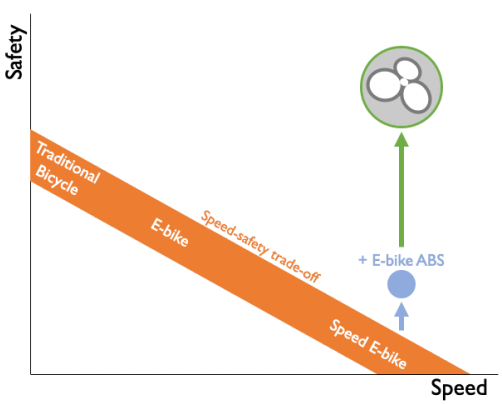
\includegraphics[width=1.1\linewidth]{images/snelheid-veiligheid-tradeoff.png}
  \caption{Snelheid-veiligheid trade-off (bron: IntuEdrive)}
  \label{fig:snelheid-veiligheid trade-off (bron: IntuEdrive)}
\end{wrapfigure}
\noindent Mobiliteit op twee wielen kennen we al lang: fietsen bestaan al sinds de 19de eeuw. Elektrische fietsen hebben het potentieel van deze tweewielers enorm verhoogd: fietsen wordt moeiteloos en stukken sneller. Spijtig genoeg neemt het risico op ongevallen ook toe bij hogere snelheid. Dat komt omdat e-bikes en speed e-bikes precies dezelfde technologie gebruiken als normale fietsen – grote wielen met smalle banden, kettingaandrijving met manuele versnellingen, mechanische handremmen – bij veel hogere snelheden. IntuEdrive noemt dit de snelheid-veiligheid trade-off. De veiligheid kan beperkt worden verhoogd door componenten toe te voegen (bv. Bosch e-bike ABS), maar de functionaliteit van deze systemen blijft beperkt. Er is een meer holistische aanpak nodig. Bovendien bieden elektrische fietsen vandaag nog niet het gebruiksgemak en de betrouwbaarheid die de consument gewend is van zijn wagen.
\\\\
IntuEdrive’s \textit{CoSaR} is een snelle elektrische fiets die veiliger is dan de klassieke mechanische fiets, dankzij hun innovatieve tweewielaandrijving en elektrische remfunctie. Dit systeem reduceert de stopafstand met 60\% en maakt schakelen overbodig (automatische versnellingen). Het stapt ook af van de onderhoudsintensieve fietscomponenten (ketting, tandwielen, mechanische remmen). Dit maakt CoSaR de perfecte e-bike voor woon-werkverkeer: makkelijk, veilig en betrouwbaar.
\\\\
Door automatisch te schakelen zorgt CoSaR ervoor dat de fietser in elke situatie precies zo snel trapt als hij of zij wil. Deze gewenste trapsnelheid – of beter trapcadans – varieert van persoon tot persoon en hangt af van omstandigheden zoals helling, tegenwind en rijsnelheid. Omdat deze gewenste cadans niet op voorhand gekend is, schakelt de transmissie momenteel op basis van een vaste wetmatigheid die tijdens testen getuned is om voor zoveel mogelijk gebruikers comfortabel aan te voelen. Wijkt deze wetmatigheid af van de gewenste cadans van een specifieke gebruiker, dan kan deze gebruiker via knoppen op het stuur tijdens het fietsen zijn of haar cadans manueel aanpassen.
\\
\begin{figure}
  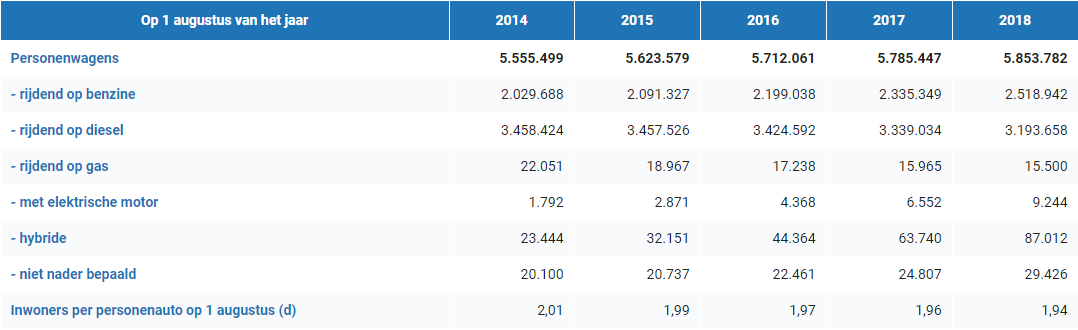
\includegraphics[width=\linewidth]{images/wagenpark_belgie.png}
  \caption{Grootte van het voertuigenpark 2014-2018 (bron: statbel.fgov.be)}
  \label{fig:wagenpark}
\end{figure}


\section{Online machine learning voor geïndividualiseerde cadanscontrole}
Deze thesis werkt verder op het prototype geleverd door IntuEdrive. Zoals reeds aangehaald schakelt de fiets automatisch. De trapcadans wordt hierdoor stabiel gehouden, ook wanneer de fietser harder of zachter trapt. Het doel is om deze instelling te veranderen door de cadans van de e-bike in real time te voorspellen aan de hand van de toestand van de fiets, zodat de trapsnelheid zich aanpast aan de huidige omstandigheden en de individuele gebruiker. Deze implementatie zal ervoor zorgen dat de fietser meer aandacht kan besteden aan de weg, waardoor gevaarlijke situaties kunnen vermeden worden. Om de cadans te personaliseren en dynamisch te maken, zal een machine learning algoritme ontwikkeld worden dat de toestand van de fiets als input binnenkrijgt en hiermee de trapsnelheid berekent. Wanneer de fietser besluit om de cadans manueel aan te passen, interpreteert het algoritme dit als een signaal om bij te leren.
\\\\
Om de performantie van het machine learning algoritme te testen zal het volledig systeem fiets-fietser-cadanscontrole gesimuleerd worden. Het fietsmodel wordt geleverd door IntuEdrive en zal geïmplementeerd worden in python. Vervolgens worden een aantal machine learning algoritmes vergeleken op basis van een aantal vooraf gedefinieerde performance indicatoren. De machine learning algoritmes zijn afkomstig uit scikit-learn, een machine learning library.
\\\\
De cadanscontrole moet aan verschillende eisen voldoen. Het algoritme moet draaien op een Raspberry Pi, samen met het controleprogramma van de fiets. Door deze beperkte resources moet het algoritme zo efficiënt mogelijk zijn. De voorspellingen moeten bijna in real time berekend worden. Het doel is om aan 10Hz de cadans aan te passen, maar hoe meer voorspellingen per seconde, hoe beter. Tragere voorspellingen kunnen hinderlijk zijn voor het rijgedrag. Ten slotte moet er ook rekening gehouden worden met de veiligheid van de fietser. Opeenvolgende voorspellingen mogen niet te veel van elkaar verschillen, anders zou de fietser erdoor gestoord kunnen worden en zijn concentratie verliezen. Bovendien mag de cadans nooit hoger dan een bepaalde maximum limiet ingesteld worden.
\\\\
De algoritmes worden geëvalueerd op basis van de mean squared error tussen de ingestelde cadans - afkomstig van het machine learning algoritme - en de zogenaamde \textit{\gls{fcc}} van de fietser. Die freely chosen cadence is niet precies gekend en wordt in de simulatie bepaald aan de hand van een fietsersmodel. Dit is een functie die de toestand van de fiets en de fietser (rijsnelheid, helling,...) afbeeldt op de trapsnelheid die de fietser in dat geval het meest comfortabel vindt. Simpel gezegd is het fietsersmodel een functie met als input de toestand van de fiets en als output een “optimale cadans”. Deze functie is speculatief en kan makkelijk aangepast worden. Op welke basis de fietser precies zijn freely chosen cadence bepaalt is voor dit onderzoek weinig relevant. Het gaat er hier vooral om dat het machine learning algoritme het fietsersmodel kan achterhalen.
\\
\begin{center}
Fietsersmodel:\tab fcc = f(snelheid,koppel,vermogen,helling,...)
\end{center}
Het algoritme moet kunnen bijleren met een kleine hoeveelheid data. De gebruiker zal immers niet vaak manuele aanpassingen doen aan de cadans. Te veel data gebruiken kan een negatieve invloed hebben op reeds correcte voorspellingen. Het algoritme moet ook snel bijleren. Elke verandering moet zo snel mogelijk doorgevoerd worden en moeten een betekenisvolle impact hebben.
\section{Huidige systeem}
De fiets van intuEdrive gebruikt een elektrische \gls{cvt} die ervoor zorgt dat er naadloos geschakeld kan worden tussen versnellingen, in tegenstelling tot het traditionele ketting-en-tandwiel systeem. Dit oude systeem schakelt in discrete trappen, waardoor de fietser tijdens het schakelen een discontinuïteit voelt. Het CVT-systeem gebruikt 2 motoren en schakelt traploos. Eén van de motoren regelt de trapcadans, de andere motor regelt het ondersteuningsniveau. Het ondersteuningsniveau bepaald hoeveel extra elektrisch vermogen er geleverd wordt, bovenop wat de fietser zelf levert.
\\\\
Figuur \ref{fig:Blokdiagram van het fiets-fietser-controller systeem} toont een blokdiagram van het systeem fiets-fietser-controller. We gaan ervan uit dat de fietser op elk moment een bepaalde referentiesnelheid (\gls{v_ref}) probeert te halen, hier aangeduid met \gls{r}. Deze kan variëren naar gelang de situatie, maar is voor elke gebruiker anders. Tijdens het fietsen geeft de fietser input aan de fiets (\gls{u_cy}). Zo kan hij of zij het geleverde koppel variëren (\gls{t_cy}), i.e. meer of minder kracht op de pedalen zetten of de cadans aanpassen met de knoppen (\gls{u_c}). Inputs en fysische toestand van de fiets worden gemeten door sensoren op de fiets: het koppel (\gls{t_cy,m}), de hoek van de trapas (\gls{theta_cr}), snelheid (\gls{v_bike}), helling (\gls{helling}), etc. $T_{cy}$ en $T_{cy,m}$ zijn niet hetzelfde, want er kunnen fouten gebeuren tijdens het meten. De vector van meetwaarden (\gls{y}) is input voor de fietscontroller. De fietscontroller stuurt de motoren in de E-bike aan (\gls{u_contr}) op basis van de metingen $y$ en de ingestelde referentiecadans. De cadanscontroller die in deze thesis uitgewerkt zal worden zal op basis van dezelfde metingen een gepersonaliseerde referentiecadans (\gls{fcc_est}) voorspellen die als input dient voor de controller.
\tikzset{
block/.style = {draw, fill=white, rectangle, minimum height=3em, minimum width=9em},
tmp/.style  = {coordinate}, 
input/.style = {coordinate},
output/.style= {coordinate},
box/.style={draw=gray,dashed,fill opacity = 0,thick,inner sep=5pt},
test/.style = {}
}
\begin{gather*}
r = \begin{bmatrix}
       v_{ref}  
     \end{bmatrix} \tab
u_{cy} = \begin{bmatrix}
       T_{cy} \\ u_c  
     \end{bmatrix} \tab
cc = \begin{bmatrix}
       FCC_{est}  
     \end{bmatrix} \tab
y = \begin{bmatrix} 
       \theta _{cr} \\ T_{cy,m} \\ v_{bike} \\ \alpha
     \end{bmatrix} 
\end{gather*}
\begin{figure}[h]
\begin{tikzpicture}[auto, node distance=2cm,>=latex']
    \node [input, name=fietsinput] (fietsinput) {};
    \node [block, right of=fietsinput,node distance=5cm] (fietser) {Fietser};
    \node [tmp, right of=fietser,node distance=3cm] (above_fietser){};
    \node [block, below of=above_fietser,node distance=3cm] (fiets) {Fiets};
    \node [tmp, left = 1.5cm of fiets] (left_fiets) {};
    \node [block, below of=fiets] (controller){Controller};
    \node [tmp, left = 1.5cm of controller] (left_controller) {};
    \node [block, below of=controller] (cadencecontroller) {Cadanscontroller};   
    \node [tmp, left = 1.5cm of cadencecontroller] (left_cadencecontrol) {};
    \node [tmp, right of=fiets,node distance=3cm] (right_fiets){};    
    \node [tmp, right of=right_fiets] (output){};    
    \draw [->] (fietsinput) -- node{$r$} (fietser);
    \draw [->] (fietser) |- (above_fietser) -- node{$u_{cy}$} (fiets);
    \draw [->] (controller.west) |- (left_controller) |- node {$u_{contr}$} (fiets.west);
    \draw [->] (cadencecontroller) -- node{$cc$} (controller);
   	\draw [->] (right_fiets) |- (controller.east);
   	\draw [->] (right_fiets) |- (cadencecontroller.east);
    \draw [->] (fiets) -- node [name=y] {$y$}(output);   
\end{tikzpicture}
\caption{Blokdiagram van het fiets-fietser-controller systeem}
  \label{fig:Blokdiagram van het fiets-fietser-controller systeem}
\end{figure}
\\\\
\chapter{Methode}
In dit hoofdstuk worden de bouwblokken van de fietssimulatie aangehaald. Daarna bekijken we de verschillende stappen, zoals preprocessing, ..., die aanwezig zijn in de cadanscontroller. Vervolgens wordt er een stochastisch keuzemodel voorgesteld dat de willekeurigheid van een mens moet simuleren. Ten slotte worden verschillende methodes besproken die ervoor zorgen dat een model zich snel kan aanpassen.
\section{De fietssimulatie}
Er wordt een simulatie gemaakt die de toestand van de fiets zo goed mogelijk benadert. Er zal geen rekening gehouden worden met het manoeuvreren van de fiets of met tegenwind. Enkel de relevante meetwaarden worden bijgehouden. De simulatie is geparametriseerd om eenvoudig verschillende scenario’s te testen. De simulatie is gebaseerd op werk van \cite{hardware implementation}.
\\\\
Het voordeel van de fietssimulatie is de enorme flexibiliteit. Uren aan data kunnen in een mum van tijd gegenereerd worden, waardoor het makkelijk is om verschillende testen uit te voeren. Hiervoor moeten slechts enkele instellingen aangepast worden. Het is ook mogelijk om slechts een enkele parameter aan te passen tijdens testen, terwijl de rest constant blijft (\textit{ceteris paribus}), wat praktisch onmogelijk is in een veldtest. Omdat de simulatie bovendien een duidelijke referentie genereert voor de FCC (output van het fietsersmodel), kan de performantie van de cadanscontroller op een kwantitatieve manier worden geëvalueerd. Tijdens een veldtest zou de fietser alleen kwalitatief kunnen aangeven of hij of zij de voorspelde cadans goed vindt. 
\subsection*{Modelleren van het fietserkoppel}
Het fietserkoppel wordt gemodelleerd als een sinusfunctie met twee pieken per omwenteling van de trapas (2 benen), met het DC-koppel van de fietser als parameter. \gls{dc} binnen de signaaltheorie wordt gezien als het signaal op nul Hertz. Het DC-koppel is vergelijkbaar met het gemiddeld koppel.
\\
\begin{gather*}
 T_{cy} = \gls{t_dc}(1+sin(2\theta_{cr}-\frac{\pi}{6}))
\end{gather*}
\\
Uit deze formule is het ook meteen duidelijk dat het DC-koppel ook het vermogen-equivalent koppel is. Dat wil zeggen dat het DC-koppel gedurende een volledige omwenteling van de trapas evenveel arbeid levert als het fietserkoppel.
\\
\begin{align*}
\int_{0}^{2\pi} T_{cy}(1+sin(2x-\frac{\pi}{6})) dx &= T_{cy} \int_{0}^{2\pi}(1+sin(2x-\frac{\pi}{6})) dx\\
&= T_{cy} \left[x-\frac{1}{2}sin(\frac{1}{3}(6x+\pi))\right]_0^{2\pi}\\
&= 2\pi \ T_{cy}
\end{align*}
\\
\noindent
Het gemiddelde koppel geleverd door de fietser wordt gemodelleerd als een proportionele regelaar. Het doel is om een bepaalde snelheid, $v_{ref}$, te behalen. Hoe groter het verschil is tussen de referentiesnelheid en de eigenlijke snelheid, hoe meer kracht er geleverd zal worden. Als deze referentiesnelheid overschreden wordt, dan zal er geen koppel meer geleverd worden. Dit wordt ook wel \textit{freewheelen} genoemd. Om de kracht van de actor te limiteren, wordt er een maximum koppel ingesteld ($T_{dc,max}$) naar gelang de huidige cadans (\gls{omega_cr}). Zo wordt er meer kracht geleverd wanneer de cadans laag is, net zoals in de werkelijkheid. \gls{k} bepaalt de agressiviteit van de regelaar. De formules zien er als volgt uit:

\begin{gather*}
\gls{t_dc_max} = \frac{-\omega_{cr}}{2}+60 \tab (Figuur\ \ref{fig:koppeltoerentalkarakteristiek}) \\
T_{dc} = min(T_{dc,max},max(0,-K*(v_{bike}-v_{ref}))
\end{gather*}
\\
\begin{figure}
  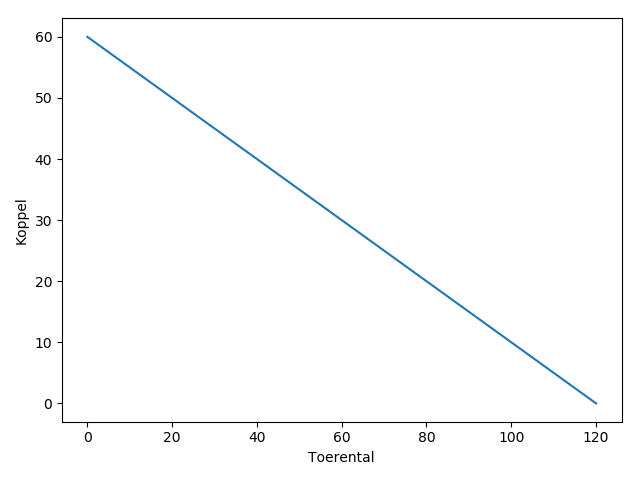
\includegraphics[width=\linewidth]{images/koppel-toerentalkarakteristiek.png}
  \caption{De koppel-toerentalkarakteristiek}
  \label{fig:koppeltoerentalkarakteristiek}
\end{figure}
\\
\noindent Figuren \ref{fig:menselijkkoppelverloop} en \ref{fig:gesimuleerdkoppelverloop} tonen een menselijk koppelverloop en gesimuleerd koppelverloop, gesampled aan 10 Hz. Zoals te zien is het gesimuleerde koppel heel consistent. Het menselijk koppel volgt duidelijk een cyclische functie, maar vertoont vormen van inconsistentie. Merk wel op dat er telkens een afwisseling is van een hoge en een lage piek. Dit wijst op een dominant been. Figuur \ref{fig:gesimuleerde koppel dominant been} toont een gesimuleerd koppelverloop van een fietser met een dominant been.
\\\\
\begin{figure}[t!]
\centering
\begin{subfigure}{.5\textwidth}
  \centering
  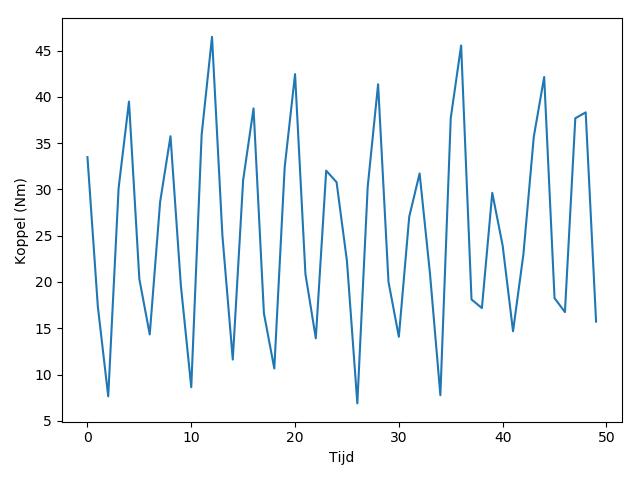
\includegraphics[width=\linewidth]{images/menselijkkoppel.png}
  \caption{Menselijk koppelverloop}
  \label{fig:menselijkkoppelverloop}
\end{subfigure}%
\begin{subfigure}{.5\textwidth}
  \centering
  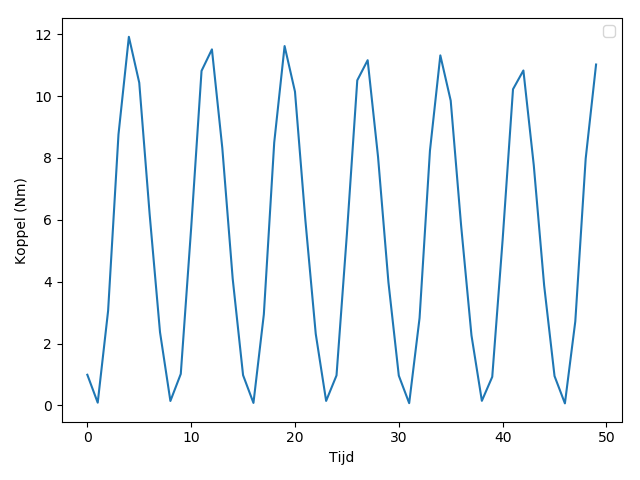
\includegraphics[width=\linewidth]{images/gesimuleerdekoppel.png}
  \caption{Gesimuleerd koppelverloop}
  \label{fig:gesimuleerdkoppelverloop}
\end{subfigure}
\begin{subfigure}{.5\textwidth}
  \centering
  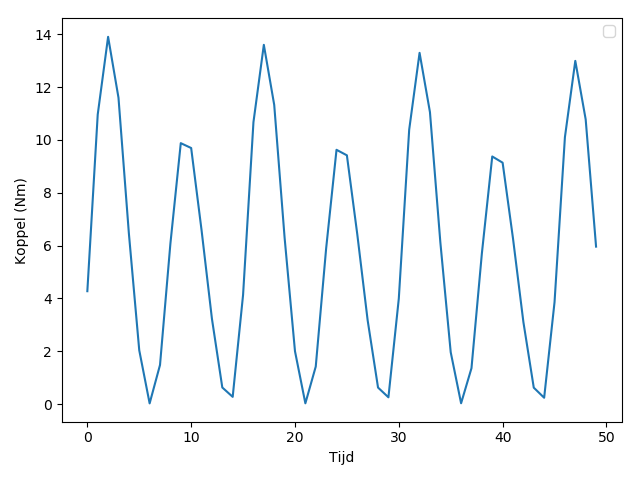
\includegraphics[width=\linewidth]{images/gesimuleerdekoppeldominantbeen.png}
  \caption{Gesimuleerd koppelverloop met dominant been}
  \label{fig:gesimuleerde koppel dominant been}
\end{subfigure}
\caption{Het koppelverloop van een mens (linksboven), de simulatie (rechtsboven) en een gesimuleerd dominant been (onderaan)}
\label{fig:koppelverloop mens-simulatie}
\end{figure}
\newpage
\begin{wrapfigure}{R}{0.5\textwidth}
  \centering
  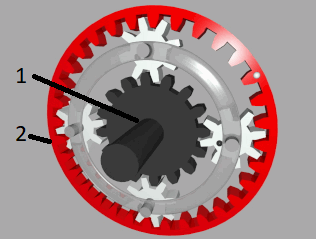
\includegraphics[width=\linewidth]{images/planeetwielmechanisme.png}
  \caption{Planeetwielmechanisme (bron: Wikipedia)}
  \label{fig:planeetwielmechanisme}
\end{wrapfigure}

\noindent $T_{cy}$ is het koppel op de trapas. Dit moet nog overgebracht worden op het achterwiel. Ellio maakt gebruik van een planeetwielmechanisme (figuur \ref{fig:planeetwielmechanisme}). Dit mechanisme laat toe om een grote overbrengingsverhouding te voorzien in een kleine ruimte. Het achterwielkoppel wordt beïnvloed door het aantal tanden op het zonnewiel (1; \gls{ns}) en het ringwiel (2; \gls{nr}) en de overbrengingsverhouding tussen de trapas en het ringwiel (\gls{k_cr,r}). Het koppel op het achterwiel (\gls{t_rw}) ziet er als volgt uit:
\begin{gather*}
T_{rw}=T_{cy}*k_{cr,r}*\frac{nr+ns}{nr}
\end{gather*}
\\\\
Bovenop het vermogen geproduceerd door de fietser, levert Ellio extra ondersteuning a.d.h.v. een motor (\gls{t_mg2}) gekoppeld aan het voorwiel. De fietser kan zelf een ondersteuningsniveau (\gls{s}) instellen tussen 0 en 5. Hoe hoger dit ondersteuningsniveau, hoe minder inspanning de fietser moet leveren. 
\begin{gather*}
T_{MG2}=min(35,S\thinspace .\thinspace T_{cy})
\end{gather*}

\subsection*{Het fietsersmodel}
Hoe kiest een fietser zijn cadans? Dit is voor elke fietser verschillend en er is nog nauwelijks onderzoek naar gebeurd. Wielrenners trainen om sneller te kunnen trappen omdat dit efficiënter is. Ze kunnen een gemiddeld vermogen leveren van 300 Watt. De doorsnee fietser levert gemiddeld ongeveer 75 Watt tijdens een normale fietstocht. Het fietsersmodel zal hierop worden afgesteld, aangezien wielrenners niet de voornaamste doelgroep zijn voor Ellio.
\\\\
Het fietsersmodel is een functie die op verschillende manieren uitgedrukt kan worden: op basis van de helling, gemiddeld koppel, of snelheid. Wat het correcte model is, wordt in deze thesis niet uitgewerkt. Het is vooral van belang dat de cadanscontroller het model zo snel en zo nauwkeurig mogelijk kan achterhalen, ongeacht wat het model precies is. Hier wordt de volgende aanname gemaakt: hoe hoger het koppel geleverd door de fietser, hoe hoger de gewenste cadans. Wanneer de fietser bijvoorbeeld een helling oprijdt, schakelt hij of zij een versnelling omlaag zodat de kracht die op de pedalen gezet moet worden aangenaam blijft. We stellen hier volgende eenvoudige modellen voor:
\begin{align*}
Gemiddeld \ koppel:\tab FCC &= \gls{f_k} . T_{dc}\\
Helling:\tab FCC &= \gls{f_h} . \alpha\\
Snelheid:\tab FCC &= \gls{f_v} . v_{bike}
\end{align*}
Er wordt verder aangenomen dat de fietser ook een zekere lineariteit verwacht bij lage snelheden (figuur \ref{fig:cadansverloop}). Dat wil zeggen dat een fietser het niet comfortabel vindt wanneer hij of zij snel moet trappen wanneer de fiets nog stilstaat of heel traag rijdt, ook al moet er op dat moment veel koppel geleverd worden om te kunnen vertrekken. Daarom wordt bij lage snelheden de FCC begrensd door een lineair oplopend maximum, te vergelijken met een mechanische fietsversnelling. Omdat de doorsnee fietser niet heel traag of heel snel trapt, wordt de FCC begrensd tussen de 40 en 120 rpm.
\begin{figure}
  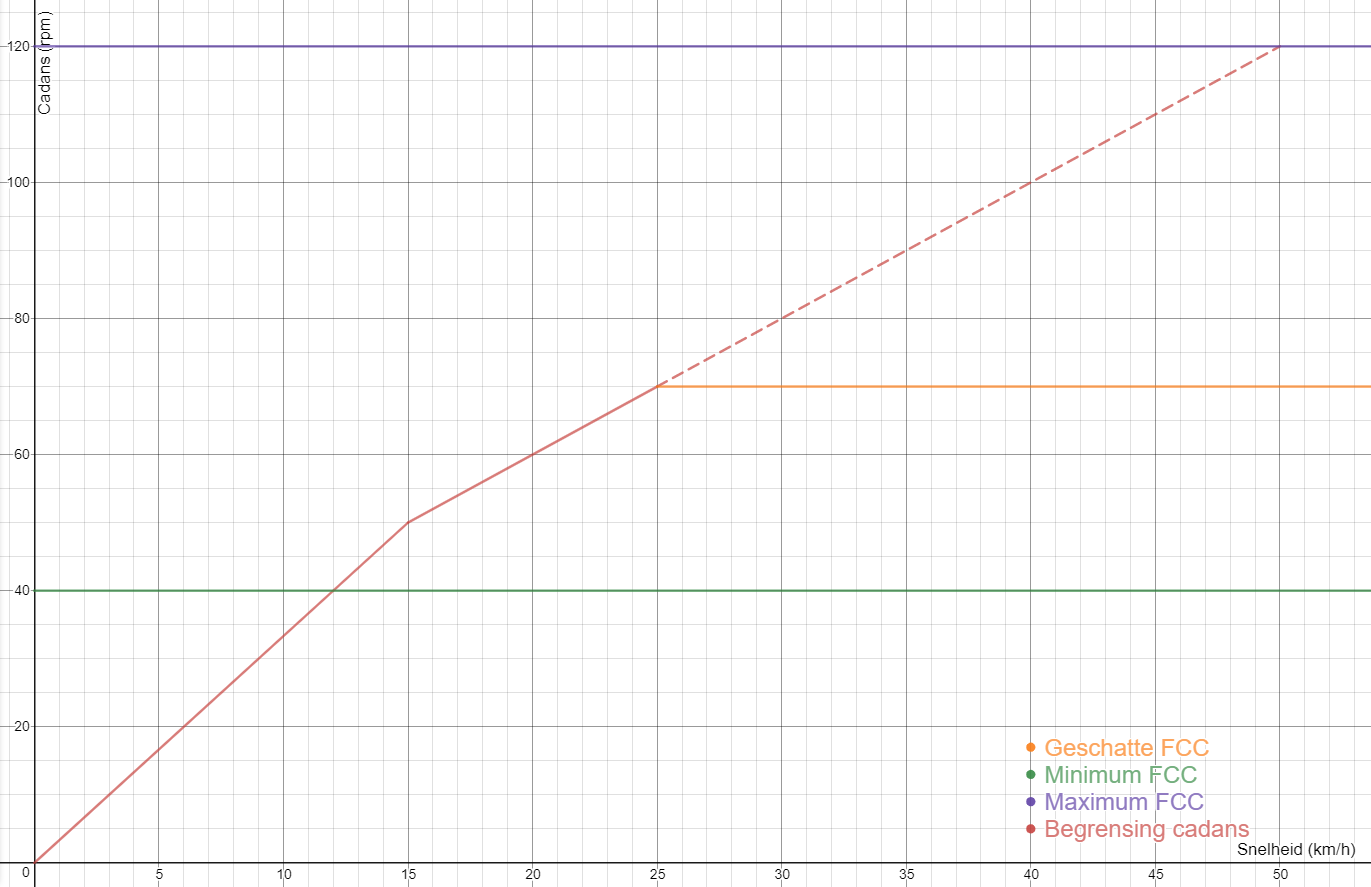
\includegraphics[width=\linewidth]{images/cadansverloop.png}
  \caption{Verwacht cadansverloop in functie van de snelheid.}
  \label{fig:cadansverloop}
\end{figure}
\newpage
\subsection*{Het lastmodel}
De simulatie is voorzien van een lastmodel. Zoals in realiteit, werken lasten in op de fiets. Zwaartekracht, wrijving met de weg en luchtweerstand zijn gemodelleerd als volgt:
\\
\begin{align*}
\gls{f_grav}&=\gls{m} \ . \ \gls{g} \ . \ sin \ \alpha \\
\gls{f_friction}&=m \ . \ g \ . \ \gls{c_r} \ . \ cos \ \alpha \\
\gls{f_aero}&=\frac{\gls{c_d} \ . \ \gls{rho_aero} \ . \ \gls{a_aero} \ . \ v_{bike}^2}{2}
\end{align*}
Samen vormen ze de totale belasting op de fiets.
\[\gls{f_load} = F_{grav}+F_{friction}+F_{aero}\]
Deze lasten zorgen ervoor dat de simulatie een realistische hoeveelheid vermogen nodig heeft om een bepaalde snelheid te halen. Er wordt hier geen rekening gehouden met de wind. Ten eerste zou dit extra complexiteit toevoegen aan de simulatie. Ten tweede vertrekken we van volgende hypothese:
\\\\
\tab De \textit{freely chosen cadence} hangt af van de hoeveelheid last, van welke bron dan \tab ook, die de gebruiker ondervindt.
\\\\
Het voorgestelde lastmodel omvat deze vereiste. Door de helling en referentiesnelheid te variëren ondergaat de fietser een veranderende last. Zoals in de realiteit zoeken mensen een bepaalde snelheid te halen. Wanneer de fietser een te hoge last ondervindt, bijvoorbeeld door een berg op te rijden, moet hij of zij meer vermogen genereren om zijn of haar gewenste snelheid te behouden. Hiervoor zijn 2 mogelijkheden: het verhogen van het koppel of de trapsnelheid. Mensen zijn meer geneigd om hun gewenste cadans te behouden, ongeacht het koppel (binnen bepaalde grenzen). De formule voor mechanisch vermogen gaat als volgt:
\[\gls{p}=T_{cy} \ . \omega_{cr} \]
Om het lastmodel correct te laten werken, moet er nog een helling gegenereerd worden. Om veel werk uit te sparen met het uitstippelen van parcours, wordt dit dynamisch gegenereerd met behulp van \textit{Perlin noise} (figuur \ref{fig:hellingverloop}). Perlin noise kan gebruikt worden om willekeurige getallen te genereren waarbij opeenvolgende getallen weinig van elkaar verschillen. Een perfecte kandidaat dus om terrein te simuleren. Om verschillende trajecten te creëren, kan de seed variabele aangepast worden. Een hellingsgraad wordt in de fietswereld vaak percentueel voorgesteld. Deze implementatie heeft echter radialen nodig. De helling zal beperkt worden tussen $\approx$ 0 en 10\% (0 en 0.1 radialen). Ter vergelijking, de Koppenberg heeft een gemiddeld stijgingspercentage van 11.6\%. Het minimum stijgingspercentage is zo gekozen dat de simulatie zo weinig mogelijk gaat freewheelen.
\begin{figure}[t]
  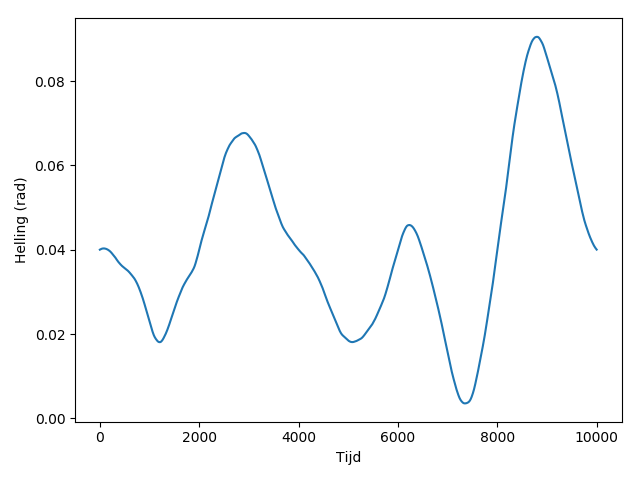
\includegraphics[width=\linewidth]{images/parcour_slope_example.png}
  \caption{Voorbeeld helling verloop}
  \label{fig:hellingverloop}
\end{figure}
\newpage
\subsection*{Snelheidsvergelijking}
\noindent De snelheid wordt geïntegreerd met een voorwaartse Euler methode. De acceleratie is een functie van de last, het totaalgewicht (m), het koppel geleverd door de fietser op het achterwiel ($T_{rw}$) en het koppel van een motor bevestigd op het voorwiel ($T_{MG2}$). 
\\\\
De bewegingsvergelijking van de fiets is, met inbegrip van het lastmodel en het fietsersmodel:
\[F \ = \  m \ . \ a \]
Deze vergelijking wordt elke tijdsstap geïntegreerd met behulp van een voorwaartse Euler methode:
\[F = m.(\frac{v_{bike}[h]-v_{bike}[h-1]}{\Delta t})\]
\[ \frac{F.\Delta t}{m}=v_{bike}[h]-v_{bike}[h-1]\]
\[v_{bike}[h]=v_{bike}[h-1]+\Delta t .\frac{1}{m}.F\]
\[v_{bike}[h] \ = \ v_{bike}[h-1] \ + \Delta t  \ . \frac{1}{m} \ . \ (\frac{T_{MG2} \ + \ T_{rw}}{r_w} \ - \ F_{load})\]
\newpage
De volledige simulatie ziet er als volgt uit:
\begin{algorithm}
\caption*{Fietssimulatie}
\For{$\text{h} = 1,\#tijdssprongen$}
{
$T_{dc,max} = \frac{-\omega_{cr}[h-1]}{2}+60$\\
$T_{dc} = min(T_{dc,max}, \ max(0,-K*(v_{bike}[h-1]-v_{ref})))$\\
$FCC = f(T_{dc})$\\
$\omega_{cr}=cadans(v_{bike}[h-1], \ T_{dc}, \ fcc)$\\
$\theta_{cr}=\theta_{cr}[h-1] + \Delta t \ . \ \omega_{cr}$ \\
$T_{cy} = T_{dc}(1+sin(2\theta_{cr}-\frac{\pi}{6}))$\\
$T_{rw}=T_{cy}*k_{cr,r}*\frac{nr+ns}{nr}$\\
$T_{MG2}=min(35, \ S \ . \ T_{cy})$\\
$F_{grav}=m \ . \ g \ . \ sin \ \alpha$\\
$F_{friction}=m \ . \ g. \ c_r \ . \ cos \ \alpha$\\
$F_{aero}=\frac{c_d \ . \ \rho_{aero} \ . \ A_{aero} \ . \ v_{bike}[h-1]^2}{2}$\\
$F_{load} = F_{grav}+F_{friction}+F_{aero}$\\
$v_{bike} \ = \ v_{bike}[h-1] \ + \Delta t  \ . \frac{1}{m} \ . \ (\frac{T_{MG2} \ + \ T_{rw}}{\gls{r_w}} \ - \ F_{load})$
}
\end{algorithm}

\section{Voorspellen van de cadans}
Een groot deel van de toestand van de fiets wordt berekend. Om een efficiënt algoritme te creëren moet enkel de relevante data bekeken worden. Zo worden de volgende attributen gebruikt: snelheid, koppel, hoek van de trapas en helling. 
\\

\begin{wrapfigure}{R}{0.40\textwidth}
  \centering
  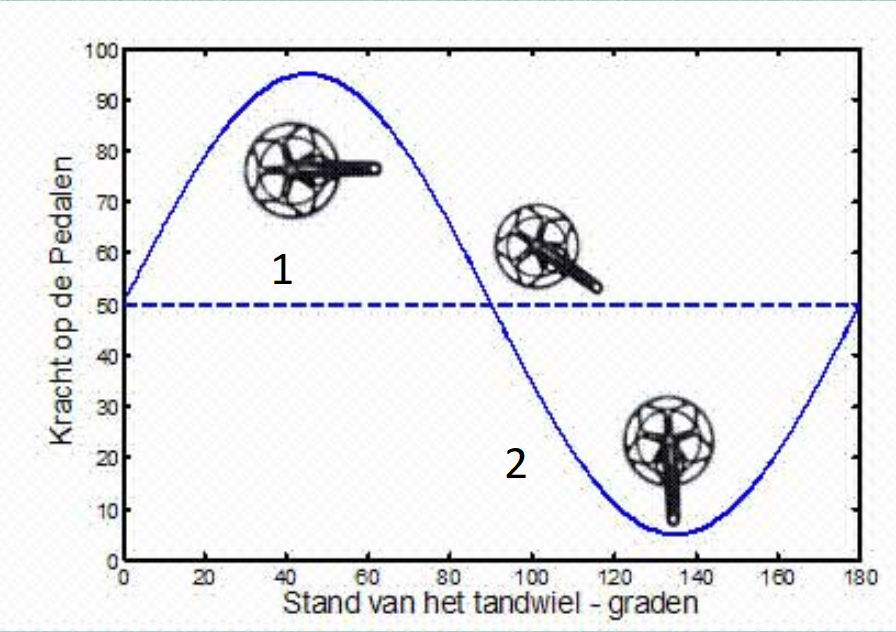
\includegraphics[width=\linewidth]{images/trapcyclus.png}
  \caption{Evolutie koppel in functie van hoek trapas (bron: fietsica.be)}
  \label{fig:Evolutie koppel in functie van hoek trapas}
\end{wrapfigure}
\noindent De helling is vanzelfsprekend. Dit is de voornaamste vorm van last en zal dus een impact hebben op de freely chosen cadence van de fietser. De hoek van de trapas en het koppel hebben individueel niet veel betekenis. Er kan bijvoorbeeld een koppel geleverd worden van 20Nm. Dit koppel kan op verschillende plaatsen geleverd worden in de trapcyclus. Als dit in de situatie 2 in figuur \ref{fig:Evolutie koppel in functie van hoek trapas} geleverd wordt, dan is dit waarschijnlijk het laagste koppel in de trapcyclus. Wordt dit geleverd gedurende de neergaande beweging (1), dan is dit het hoogste koppel. Deze verschillende situaties zullen een verschillende cadans nodig hebben. Tijdens de eerst situatie wordt er gemiddeld meer koppel geleverd, wat wijst op een grote last. Dus verwachten we hier een hoge cadans. De tweede situatie daarentegen zal gemiddeld een lagere last hebben. Daarom wordt in conjunctie met het koppel de hoek van de trapas gebruikt. Snelheid is ook een relevant attribuut. In situaties met verschillende snelheden en dezelfde last gaat de cadans verschillen.
\subsection*{Preprocessing}
Niet elk algoritme heeft nood aan genormaliseerde input. Voor algoritmes die een afstandsfunctie gebruiken is standaardisatie cruciaal. De doelvariabelen daarentegen moet niet genormaliseerd worden volgens Warren S. Sarle \cite{preprocessing faq}. In zijn FAQ schrijft hij dat het standaardiseren van de output voornamelijk voordelige effecten heeft op de initiële gewichten. Wanneer er meerdere doelvariabele zijn en als deze ver uit elkaar liggen, kan het wel nuttig zijn om ze te normaliseren. In dit geval is dat niet nodig aangezien enkel de cadans voorspeld zal worden.
\\\\
\noindent Ten eerste zal de data in sequentie gegoten worden. Een sequentie wordt gezien als een aantal vectoren ($x_t$) over verschillende tijdstippen. Een enkele data meting op zich is niet genoeg om een accurate voorspelling te maken, maar te veel data gebruiken is ook niet goed aangezien de voorspellingen tijdig moeten geleverd worden.
\\
\begin{gather*}
x_t = \begin{bmatrix} 
       \theta _{cr} \\ T_{cy,m} \\ v_{bike} \\ \alpha
     \end{bmatrix} \tab
sequentie = \begin{bmatrix} 
       x_t \\ x_{t-1} \\ ... \\ x_{t-n}
     \end{bmatrix} 
\end{gather*}
\\
\noindent Ten tweede zal de hoek van de trapas niet in zijn zuivere vorm gebruikt worden. De hoek van de trapas is een variabele tussen nul en $2 \pi$. Het probleem hier is dat het begin en het einde van een cyclus ver uit elkaar liggen. Voor de mens is het evident dat nul en twee pi hetzelfde zijn, maar voor de computer is dit een groot verschil. Daarom zal de sinus en de cosinus van de hoek genomen worden, zodat het begin en einde dicht bij elkaar liggen (figuur \ref{fig:preprocessing hoek trapas}). Zo leren we het algoritme bij dat de data zich cyclisch gedraagt.

\begin{figure}[h]
  \centering
  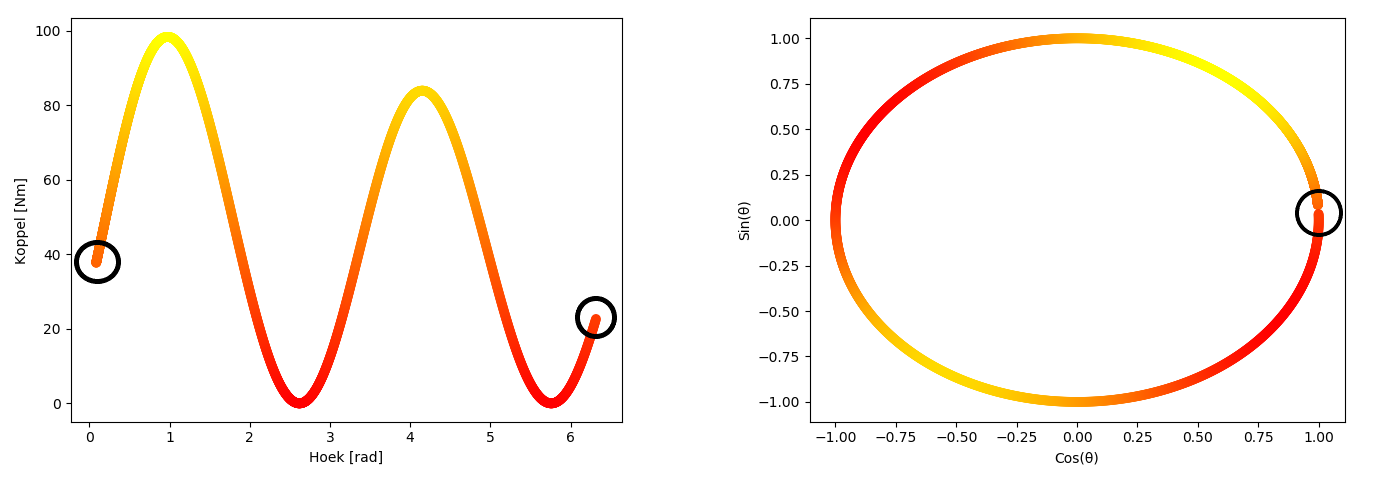
\includegraphics[width=\linewidth]{images/preprocessing-hoek.png}
  \caption{Figuur links toont dat het begin en einde van een trapcyclus ver uit elkaar liggen. Figuur rechts toont dat beide punten van de linkse figuur dicht bij elkaar liggen.}
  \label{fig:preprocessing hoek trapas}
\end{figure}

\noindent Ten slotte kan er ruis zitten op de metingen. Er zal altijd wel een klein foutje zitten op de data omdat de meetapparatuur niet perfect is. Het is mogelijk dat trillingen van de motor of het wegdek een impact kunnen hebben, voornamelijk op het geleverde koppel. Voor deze iteratie zal hier geen rekening mee gehouden worden. Ruis van het wegdek komt voor op een frequentie van ongeveer 20 Hz en hoger. Dit kan nog correct opgenomen worden als er op voorhand data wordt gesampled op hogere frequentie. Ruis van de motoren daarentegen komt voor op 13000 Hz, ver boven de sample frequentie en zal dus afgebeeld worden op lagere frequenties. Het huidige systeem zal geen rekening houden met beide soorten ruis. Om de gevoeligheid voor ruis te minimaliseren kan het ingangssignaal eenvoudig gefilterd worden met een laagdoorlaatfilter van bijvoorbeeld 10 Hz. Figuur \ref{fig:fft fietser} toont een \textit{fast fourier transformatie} van het menselijk koppelverloop.

\begin{figure}[h]
  \centering
  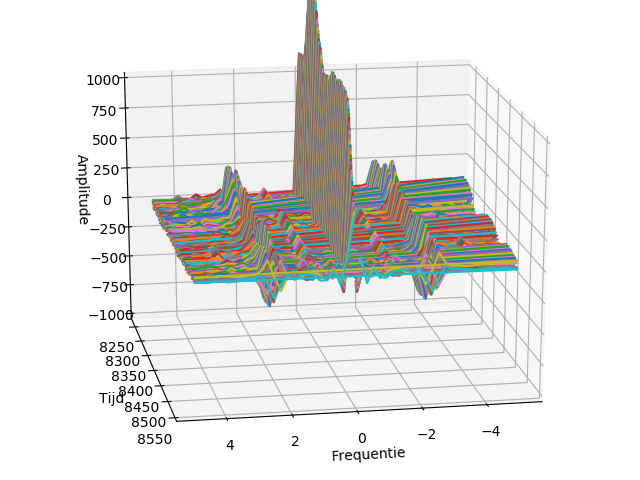
\includegraphics[width=\linewidth]{images/fft_fietser.png}
  \caption{Een Fast Fourier Transformatie van het menselijk koppelverloop.}
  \label{fig:fft fietser}
\end{figure}

\subsection*{Algoritmes}
\subsubsection*{Passive Aggressive algorithm}
Het \gls{pa} algoritme, beschreven in de paper van Crammer et al. \cite{pa algorithm}, is een on-line algoritme gelijkaardig aan een perceptron. Net zoals de perceptron, doet PA de matrixvermenigvuldiging $y_t=w_t \cdot x_t$ om de voorspelling te berekenen. Het grootste verschil tussen beide is hoe de gewichten geüpdatet worden. Het PA algoritme is bruikbaar voor classificatie, regressie, uniclass voorspellingen en multiclass problemen.
\\\\
\noindent Het PA algoritme, zoals de naam weggeeft, kan zich zowel passief als agressief gedragen. Het trainen van PA bestaat uit twee stappen. In de eerste stap wordt er een voorspelling $y_{t,p}$ gemaakt a.d.h.v. de input vector $x_t$ en gewichtenmatrix $w$. Hierna wordt het echte label $y_t$ bekendgemaakt. Als de fout kleiner is dan een voorgedefinieerde waarde $\epsilon$, dan zullen de gewichten niet geüpdatet worden. Als de error toch groter is dan deze marge, dan zullen de gewichten $w$ aangepast worden zodat de fout voor de huidige instantie nul wordt. PA past de gewichten aan zodat het verschil tussen het vorige gewicht en het nieuwe gewicht minimaal is. 
\[
    loss_{\epsilon} (w_t;(x_t,y_t))=\left\{
                \begin{array}{ll}
                  0 \tab \tab \tab \ \ |w \cdot x - y| \leq \epsilon \\
                  |w \cdot x - y| - \epsilon \tab anderzijds
                \end{array}
              \right.\\
\]
\[
    w_{t+1}= \argmin_{w \in \mathbb{R}^n}
     \frac{1}{2}||w-w_t||^2 \tab zodat \ loss_{\epsilon} (w_{t+1};(x_t,y_t)) = 0
\]
Door de agressiviteit van het standaard PA algoritme kunnen er problemen ontstaan wanneer er veel ruis zit op de data. Daarom heeft Crammer et al. twee extra versies, PA-I en PA-II, gemaakt die dit probleem oplossen. Beide versies voegen een slack variabele $\xi$ toe. Deze variabele zorgt ervoor dat bij het aanpassen van de gewichten, de fout kleiner of gelijk moet zijn aan $\xi$ in plaats van nul. Beide versies hebben ook een agressiviteits parameter C die deze $\xi$ beïnvloedt. Dit is een vorm van regularisatie om overfitting te voorkomen.

\[
   PA-I \tab w_{t+1}= \argmin_{w \in \mathbb{R}^n}
     \frac{1}{2}||w-w_t||^2 + C\xi \tab zodat \ loss_{\epsilon} (w_{t+1};(x_t,y_t)) \leq \xi
\]
\[
   PA-II \tab w_{t+1}= \argmin_{w \in \mathbb{R}^n}
     \frac{1}{2}||w-w_t||^2 + C\xi^2 \tab zodat \ loss_{\epsilon} (w_{t+1};(x_t,y_t)) \leq \xi
\]

De nieuwe gewichtenmatrix $w_{t+1}$ wordt als volgt berekend:
\[
w_{t+1}=w_t+ \tau_t y_t x_t
\]
\begin{align*}
\tau_t &= \frac{loss_t}{||x_t||^2} \tab \tab (PA)\\
\tau_t &= min \{ C, \frac{loss_t}{||x_t||^2} \} \ \ (PA-I)\\
\tau_t &= \frac{loss_t}{||x_t||^2+\frac{1}{2C}} \tab (PA-II) 
\end{align*}


\subsubsection*{Decision Tree en Random Forest}
Een \gls{dt} is een regel-gebaseerd model (\textit{rule-based model}). Dit algoritme is snel (\textit{greedy}), maar kan niet goed om met ruis. Dit model is gekend om makkelijk te overfitten. Daarom wordt het \gls{rf} algoritme simultaan bekeken.
\\\\
Een DT is een binaire boom. In elke knoop wordt een binair keuzepunt gemaakt op basis van een attribuut. Dit keuzepunt is gekozen zodat de data optimaal gesplitst is over beide takken. \texttt{Sci-kit learn} biedt de mogelijkheid aan om de maximum diepte van de boom te beperken. Wanneer deze parameter niet ingesteld is, zal de DT blijven groeien totdat alle blad nodes ``puur" \ zijn. Een correcte diepte kiezen is een enorm moeilijke taak.
\\\\ 
RF is een ensemble. Dit wilt zeggen dat meerdere algoritmes, in dit geval meerdere DT’s, gebruikt worden om een betere voorspelling te maken. L. Breiman \cite{randomforest paper} beweert in zijn paper dat alle RF’s convergeren zodat overfitting geen probleem is. In tegenstelling tot DT’s, kiest een RF geen optimaal attribuut wanneer een node gesplitst wordt. De variabele worden at random gekozen, waardoor geen enkele boom dezelfde is. De verschillende bomen trainen niet met exact dezelfde trainingsdata. Ze passen Bootstrap Aggregating toe, of bagging. Dit houdt in dat uit de originele trainingsset data wordt gesampled at random. Een instantie kan meerdere keren gesampled worden. Deze techniek reduceert de variantie.
\subsection*{Post-processing}
De cadans variëert lichtjes doorheen een trapcyclus, zowel in het echt als in de simulatie. De voorspellingen zullen dezelfde trend vertonen. Bovendien kan een beetje ruis of het gedrag van de fietser voor afwijkingen zorgen, bijvoorbeeld een grote sprong tussen twee voorspellingen. Dit kan ergerend zijn voor de fietser.
\\\\
Dit probleem kan op verschillende manieren opgelost worden. Gebruikmakend van de huidige en vorige voorspellingen (\gls{fcc_pred}) of de vorige schatting ($FCC_{est}$). De vorige instelling is de cadans die is doorgegeven aan de fiets controller.
\begin{align*}
\gls{ma} \tab  FCC_{est,t} &= \frac{\sum_{i=0}^{n} FCC_{pred,t-i} }{n}\\
\gls{es} \tab FCC_{est,t} &= \gls{sf} . FCC_{pred,t} + (1-sf) . FCC_{est,t-1}
\end{align*}
MA lost beide problemen goed op. Meer voorspellingen leidt tot stabielere schattingen, maar dit introduceert een vertraging (\textit{lag}) op de cadans. Namelijk wanneer de omstandigheden veranderen, zal de ingestelde cadans slechts na enkele iteraties optimaal zijn, in plaats van onmiddellijk. ES vermindert de amplitude van de oscillaties slechts in mindere mate. Figuur \ref{fig:effecten postprocessing} toont wat de impact is van ES en MA op ruizige voorspellingen (20\% kans op ruis tussen -10 en +10).
\begin{figure}[!t]
\centering
\begin{subfigure}{.5\textwidth}
  \centering
  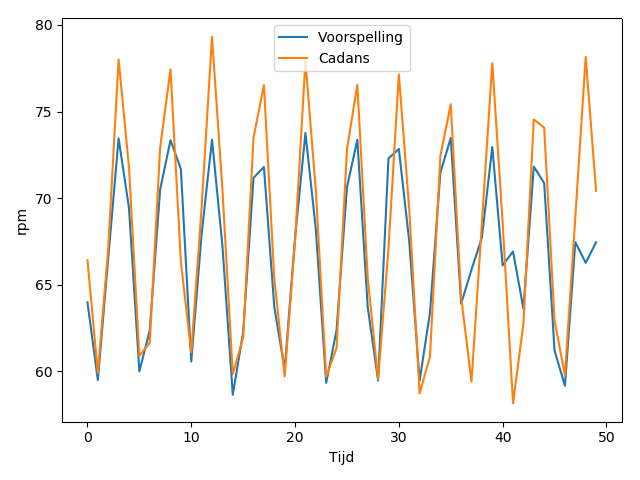
\includegraphics[width=\linewidth]{images/actual-prediction+noice,nopp.png}
  \caption{Geen post-processing}
  \label{fig:geen postprocessing}
\end{subfigure}%
\begin{subfigure}{.5\textwidth}
  \centering
  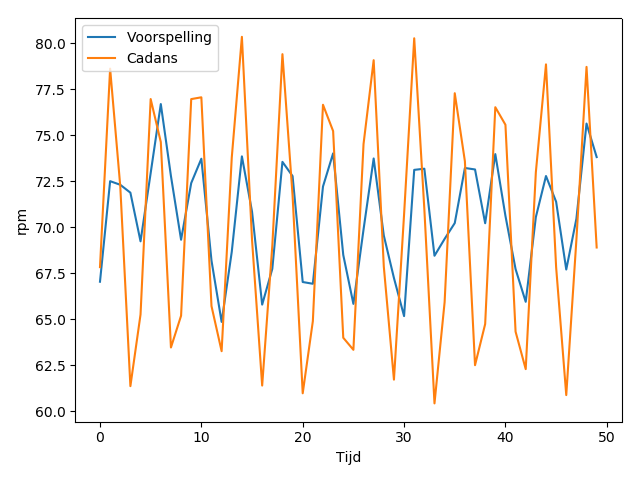
\includegraphics[width=\linewidth]{images/actual-prediction+noice,es.png}
  \caption{Exponential Smoothing}
  \label{fig:exponential smoothing postprocessing}
\end{subfigure}
\begin{subfigure}{.5\textwidth}
  \centering
  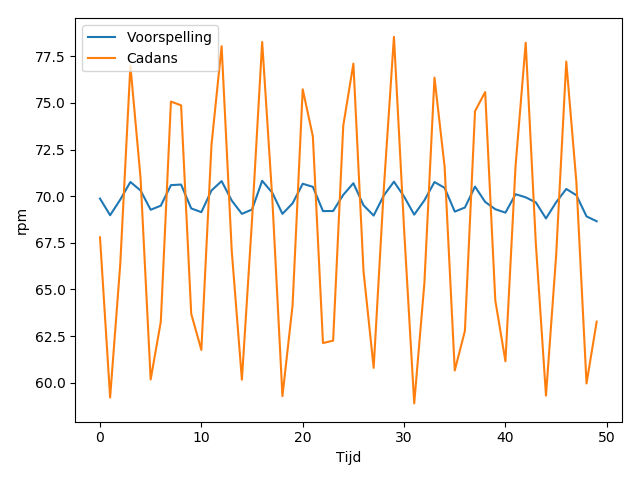
\includegraphics[width=\linewidth]{images/actual-prediction+noice,ma.png}
  \caption{Moving Average}
  \label{fig:moving average postprocessing}
\end{subfigure}
\caption{De effecten van verschillende post-processing technieken.}
\label{fig:effecten postprocessing}
\end{figure}
\newpage
\section{Stochastisch bijleren}
Het volgende hoofdstuk van deze thesis bespreekt de experimentele resultaten. In deze testen leren de algoritmes op een deterministische manier bij. Een mens daarentegen is onvoorspelbaar. Soms is de fietser snel geërgerd en drukt hij sneller op de knop om zijn cadans aan te passen. Soms vindt hij een incorrecte cadans niet erg genoeg om daarvoor op de knop te duwen. Dit zou gesimuleerd moeten worden om te achterhalen of de modellen met dit non-determinisme omkunnen. 
\\\\
Net zoals volgens de deterministische update-strategie, zal het fietsersmodel als de waarheid genomen worden. Hoe groter het absoluut verschil is tussen de cadans en het fietsersmodel (\gls{delta_c}), hoe hoger de kans dat de fietser effectief op de knop zal duwen waardoor het model kan bijleren. De probabiliteit van het bijleren, hier $P(u_c|\Delta_c)$, zal lineair evolueren. Wanneer het verschil zich bevindt tussen nul en vijf, schaalt de kans lineair mee van 0\% naar 20\% kans. Wanneer deze grens overschreden wordt, groeit de kans sneller mee tot 100\% kans wanneer het verschil groter of gelijk is aan tien (figuur \ref{fig:kansverdeling cadansupdate}). Deze strategie is bedoeld voor een simulatie gesampled aan één Hertz. Als de frequentie verhoogt naar bijvoorbeeld 10000 Hz, evolueert dit stochastische beslissingsmodel naar een deterministische, aangezien er enorm vaak een kans is op de updaten. Daarom moet $P(u_c|\Delta_c)$ nog vermenigvuldigd worden met de grootte van de tijdstap (x0,1 voor 10 Hz). Of het vermenigvuldigen van de frequentie met de probabiliteit van updaten correct is, is evident aan te tonen met behulp van de verwachtingswaarde over een binomiale verdeling (met $\Delta_c=5$) \cite{binomial wiki}:
\begin{align*}
E(u_c|\Delta_c)_{1hz} \ &=p(u_c=1|\Delta_c)_{1hz} \\
E(u_c|\Delta_c)_{1hz} \ &=0.2 \\
E(u_c|\Delta_c)_{10hz}&=10*p(u_c=1|\Delta_c)_{10hz} \\
E(u_c|\Delta_c)_{10hz}&=0.2
\end{align*}

\begin{figure}[h]
  \centering
  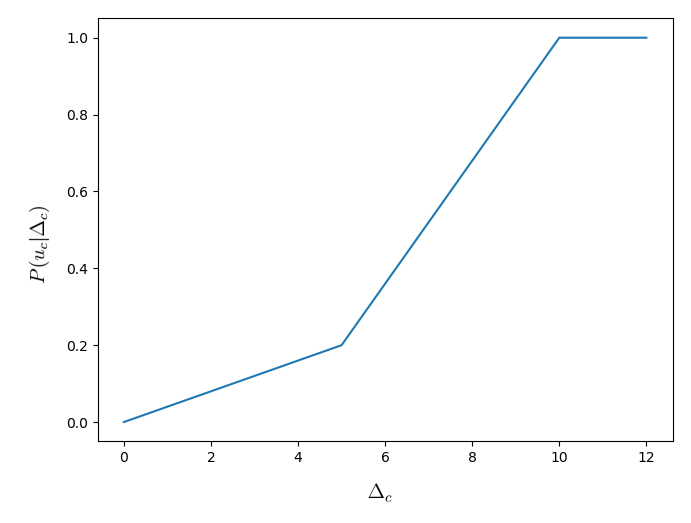
\includegraphics[width=\linewidth]{images/stochastische_kans_cadansupdate.png}
  \caption{Het verloop van de kansverdeling in functie van $\Delta_c$}
  \label{fig:kansverdeling cadansupdate}
\end{figure}

\noindent Hoe lang het gemiddeld duurt om bij te leren kan ook achterhaald worden met behulp van de verwachtingswaarde, deze keer als een geometrische distributie \cite{geometric wiki}. Het verschil tussen een binomiale distributie en een geometrische distributie is als volgt: een binomiale distributie is een kansverdeling over het aantal successen met kans $p$ na $k$ onafhankelijke testen. Een geometrische distributie vertelt iets over wat de kans is dat na $k$ pogingen, zodat de laatste poging een succes is met de kans op succes $p$ constant. Bijvoorbeeld: wat is de kans dat de simulatie na tien iteraties aan 10 Hz een update zal doorvoeren als $\Delta_c=5$?

\[p(u_c=10|\Delta_c=5)=(1-p)^9*p=0.98^9*0.02=0.01667\]
\\\\
\noindent Het gemiddeld aantal iteraties dat de simulatie nodig zou hebben om een update door te voeren, komt neer op het uitwerken van volgende oneindige reeks:
\begin{align*}
E(X)&=\sum_{k=1}^{\infty} (1-p)^kpk \\
E(X)&=p+2(1-p)p+3(1-p)^2 p...
\end{align*}
Wat neerkomt op:
\[E(X)=\frac{1}{p}\]
Voor een $\Delta_c$ van vijf zal het dus gemiddeld 5 iteraties (aan 1 Hz) en 50 iteraties (aan 10 Hz) duren vooraleer er geüpdatet wordt.
\\\\
Ten slotte wordt deze strategie beperkt, zodat het onmogelijk is om direct twee keer na elkaar op de knop te duwen. Dit is geïmplementeerd via een simpele controle van het verschil in tijd tussen de huidige iteratie en de iteratie van de vorige update.

\subsection{Verwachtingen}
We verwachten dat alle modellen dit stochastisch probleem aankunnen, omdat het verschil tussen fietsersmodel en cadans uiteindelijk groot genoeg zal worden zodanig dat het zeer onwaarschijnlijk is dat er niet op de knop geduwd wordt. Wat we hiermee willen bedoelen is dat het statistisch onwaarschijnlijk is dat er niet wordt bijgeleerd wanneer het verschil vergroot.
\section{Conceptuele drift}
Conceptuele drift is de verandering van het concept, in dit geval het fietsersmodel, na verloop van tijd. Deze verandering kan op verschillende manieren gebeuren: abrupt, geleidelijk en terugkerend. De FCC van een mens is een vorm van geleidelijke drift. Volgens Hansen et al. \cite{factors effecting cadence} heeft de leeftijd invloed op de FCC, zijnde oudere mensen trappen in het algemeen trager. De snelheid waaraan de FCC daalt, is enorm klein. Het gaat hier om drie rpm per decennium. Eens de fiets is ingesteld, zou er dus technisch gezien nooit meer moeten bijgeleerd worden, tenzij de fiets verandert van eigenaar. Dit is een vorm van abrupte drift, aangezien twee individuën hoogstwaarschijnlijk niet dezelfde FCC hebben. Deze sectie onderzoekt welke technieken er zijn om met deze abrupte drift om te gaan. Het doel van deze sectie is om een techniek te achterhalen die ervoor zorgt dat het gedrag van een tweede gebruiker zo snel mogelijk bijgeleerd is zonder de ervaring van de eerste gebruiker, die de fiets heeft gekocht, te verslechteren (het laatste is belangrijker voor IntuEdrive).
\\\\
Standaard hebben algoritmes van machinaal leren geen manier om met een drift om te gaan. Als het concept verandert, zal het nieuwe concept geleidelijk aan een groter aandeel krijgen in de trainingsset, met als gevolg dat het algoritme van machinaal leren uiteindelijk het nieuwe concept leert. Hierdoor kan het lang duren vooraleer het nieuwe concept goed voorspeld kan worden. Een techniek om met conceptuele drift om te gaan, is het vergeten van oude data (het oude concept). In dit deel zullen drie technieken besproken worden die Loeffel \cite{adaptive ml} in zijn doctoraat aanhaalt. Statisch schuivend venster (\textit{fixed sliding window}) en een sampling techniek zijn zelf geïmplementeerd zoals beschreven door Loeffel \cite{adaptive ml} en Aggarwal \cite{biased reservoir sampling} respectievelijk.
\subsection{Statisch schuivend venster (\textit{static sliding window})}
Een statisch schuivend venster is de simpelste techniek om een vergeetmechanisme toe te voegen aan een algoritme van machinaal leren voor abrupte drifts. Een statisch schuivend venster is een set van de $n$ meest recente elementen in een data stroom. Wanneer er data in het schuivend venster zit, nemen we aan dat dit het meest recente concept vertegenwoordigt. Mocht het concept plots veranderen, en het schuivend venster zit vol, dan zal de oude data plaats maken voor de nieuwe data waardoor het oude concept na verloop van tijd vergeten wordt.
\setcounter{table}{0}
\begin{table}[h]
\begin{tabular}{|c|l|}
\hline
\multicolumn{2}{|c|}{Statisch schuivend venster} \\ \hline
Voordelen & \multicolumn{1}{c|}{Nadelen} \\ \hline
\multicolumn{1}{|l|}{\begin{tabular}[c]{@{}l@{}}+ Simpel\\ + Start meteen met vergeten op het moment \\ \phantom{+} van de conceptuele drift\\ + Groot venster maakt het model robuust \\ \phantom{+} tegen ruis en zorgt voor een accuraat en \\ \phantom{+} stabiel model\\ \phantom{test} \end{tabular}} & \begin{tabular}[c]{@{}l@{}} - Een correcte grootte voor het venster \\  \phantom{-} is moeilijk te vinden\\ - Een te klein venster kan mogelijk het \\ \phantom{-} concept niet goed omvatten\\ - Een te groot venster vergeet trager\\ - Ruis kan goede, relevante data uit \\ \phantom{-} het venster verwijderen\end{tabular} \\ \hline
\end{tabular}
\caption{Voor- en nadelen van statisch schuivend venster}
\label{tab:voor- en nadelen van fixed sliding window}
\end{table}
\subsection{Variabel schuivend venster (\textit{variable sliding window})}
Een variabel schuivend venster is gelijkaardig aan een statisch schuivend venster. Het enige verschil is dat de grootte van het venster kan variëren. Dit mechanisme introduceert een veranderingsdetector (\textit{change detector}), een algoritme dat moet uitmaken of het concept verandert of niet. Als de change detector geen verandering opmerkt (zelfde concept), zal het venster vergroten. Daardoor stijgt het aantal elementen van het huidige concept. Dit brengt het voordeel met zich mee dat het model meer trainingsdata heeft en daardoor accurater en robuuster is. Eens de change detector opmerkt dat het concept verandert, dan zal de lengte van het venster verkleinen waardoor het een grote hoeveelheid data vergeet. Dit zorgt ervoor dat het model snel het nieuwe concept kan bijleren. Dit is wel een riskante strategie. De change detector kan geactiveerd worden met ruizige data (\textit{“catastrophic forgetting”}). Dit mechanisme kan bovendien ook niet goed om met een zeer trage drift, al is dit hier niet van belang. Omwille van het risico zal deze strategie niet uitgewerkt worden.

\begin{table}[!ht]
\begin{tabular}{|c|l|}
\hline
\multicolumn{2}{|c|}{Variabele schuivend venster} \\ \hline
Voordelen & \multicolumn{1}{c|}{Nadelen} \\ \hline
\multicolumn{1}{|l|}{\begin{tabular}[c]{@{}l@{}}+ Groot venster maakt het model robuust \\ \phantom{+} tegen ruis en zorgt voor een accuraat en \\ \phantom{+} stabiel model\\ + Kan venster verkleinen zodat het \\ \phantom{+} nieuwe concept snel bijgeleerd wordt\\ + Change detector kan ervoor zorgen dat\\ \phantom{+} een model hergebruikt kan worden (als\\\phantom{+} hetzelfde concept terugkeert) \\ \phantom{test}\end{tabular}} & \begin{tabular}[c]{@{}l@{}}- Een change detector implementeren is \\ \phantom{-} complex\\ - Riskante strategie\\ - Onnauwkeurige change detector zorgt voor\\ \phantom{-} problemen\\ - Change detector werkt met een drempel-\\\phantom{-} waarde voor detectie. Te klein en er kan een \\ \phantom{-} vals alarm optreden. Te groot en het zal te \\ \phantom{-} traag reageren\end{tabular} \\ \hline
\end{tabular}
\caption{Voor- en nadelen van variabel schuivend venster}
\label{tab:voor- en nadelen van variabele sliding window}
\end{table}
\newpage
\subsection{Sampling}
Ten slotte kan er gesampled worden om een relevante trainingset te genereren. Om een bias te krijgen voor recentere data zou een kansverdeling gebruikt kunnen worden met een bias naar recentere data. Dit is echter een naïeve implementatie die veel geheugen inneemt, aangezien alle trainingsdata moet bijgehouden worden. In de paper van Aggarwal C. \cite{biased reservoir sampling} worden twee technieken voorgesteld die data van een stream samplen met een bias voor recente data. Beide technieken zijn gebaseerd op reservoir sampling.

\subsubsection{Reservoir sampling}
Reservoir sampling is een sampling strategie waar er gesampled wordt uit een stream $S$. Voor elk element $x \in S$, willen we een gelijke kans hebben dat dit element $x$ gesampled wordt. Stel dat er $k$ elementen gesampled moeten worden, dan zal de probabiliteit voor elk element gelijk zijn aan $k/|S|$. Het probleem hier is dat we niet weten hoe groot $S$ precies is. Bovendien is het mogelijk dat niet alle elementen van $S$ in geheugen passen. Vitter J. \cite{reservoir sampling} lost dit op met een eenvoudig algoritme R.

\begin{algorithm}
\caption*{R}
$R = \bot \text{ met capaciteit }k$\\
$t=0$\\
\While{data stream S heeft nog elementen}
{
$t++$\\
\uIf{$t<k$}
{$A[t]=S[t]$}
\Else{
$i = random(0,t)$\\
\If{$i<=k$}
{$A[i]=S[t]$}
}
}
\end{algorithm}

\newpage
\begin{figure}[htp!]
  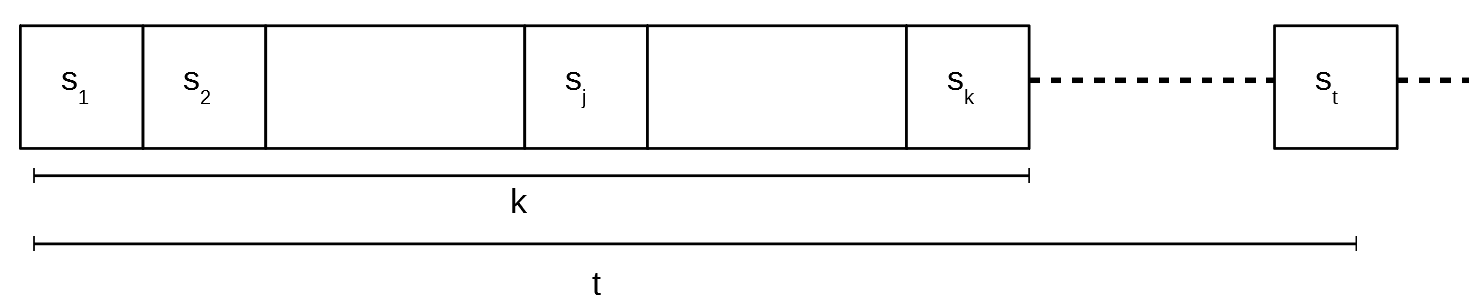
\includegraphics[width=\linewidth]{images/reservoir_sampling_voorbeeld.png}
\caption{Reservoir sampling voorstelling}
  \label{fig:reservoir sampling voorbeeld}
\end{figure}

\noindent Hypothese: $P(s_t \in R) = \frac{k}{n}$ \\
Bewijs:
\begin{align*}
P(s_t \in R) &= \frac{k}{t} * (1-\frac{1}{t+1})* (1-\frac{1}{t+2})*...*(1-\frac{1}{n}) 
\\
P(s_t \in R) &= \frac{k}{t} * (\frac{t+1-1}{t+1})* (\frac{t+2-1}{t+2})*...*(\frac{n-1}{n})
\\
P(s_t \in R) &= \frac{k}{\text{\st{t}}} * (\frac{\text{\st{t}}}{\text{\st{t+1}}})* (\frac{\text{\st{t+1}}}{\text{\st{t+2}}})*...*(\frac{\text{\st{n-1}}}{n})\\
P(s_t \in R) &= \frac{k}{n}
\end{align*}

\subsubsection{Bevoordeelde reservoir sampling (\textit{biased reservoir sampling})}
Aggarwal C. \cite{biased reservoir sampling} introduceert een bias in reservoir sampling.

\begin{algorithm}
\caption*{Bevoordeelde reservoir sampling}
$R = \bot \text{ met capaciteit }k$\\
$t=0$\\
\While{data stream S heeft nog elementen}
{
$t++$\\
$f=\text{de volheid van R, zijnde een getal tussen }[0,1]$\\
$i = random(0,1)$\\
Voeg element S[t] toe aan R\\
\If{$i<=f$}
{Verwijder een willekeurig element uit R}
}
\end{algorithm}
\noindent In zijn paper geeft Aggarwal aan dat de kans dat een element in $R$ zit exponentieel daalt in functie van $t$. Dit wil zeggen dat oudere elementen een exponentieel kleinere kans hebben om in $R$ te zitten dan recente elementen. De probabiliteit gaat als volgt, met $r$ het r-de punt in $R$, $t$ het t-de punt in S en \gls{lambda} een bias ratio die applicatie specifiek is:
\[f(r,t)=e^{-\lambda(t-r)}\]
De bias ratio $\lambda$ wordt bepaald aan de hand van de grootte van het reservoir (k):
\[\lambda=\frac{1}{k}\]

\begin{table}[!ht]
\begin{tabular}{|c|l|}
\hline
\multicolumn{2}{|c|}{Bevoordeelde reservoir sampling} \\ \hline
Voordelen & \multicolumn{1}{c|}{Nadelen} \\ \hline
\multicolumn{1}{|l|}{\begin{tabular}[c]{@{}l@{}}+ Geheugen efficiënt\\ + Kan een diverse set van data beter leren\\ \phantom{+} (data die verder uit elkaar ligt, heeft \\ \phantom{+} meer betekenis dan twee observaties vlak\\ \phantom{+} na elkaar)\\ + Het achterliggende model kan efficiënter \\ \phantom{+} worden omdat er minder data opgeslagen\\ \phantom{+} wordt\end{tabular}} & \begin{tabular}[c]{@{}l@{}}- Als het concept vaak verandert, heb je het\\ \phantom{-} ``van alles iets" \ probleem\\ - Het kan zijn dat het oude concept nog voor\\ \phantom{-} een lange tijd in het reservoir zit\\ \phantom{test} \\ \phantom{test}\\ \phantom{test}\\ \phantom{test}\end{tabular} \\ \hline
\end{tabular}
\caption{Voor- en nadelen van bevoordeelde reservoir sampling}
\label{tab:voor- en nadelen van biased reservoir sampling}
\end{table}
\newpage
\subsection{Verwachtingen}
Er wordt verwacht dat kleinere datastructuren (klein venster of reservoir), die net groot genoeg zijn om één concept te omvatten, slechter zullen presteren dan grotere datastructuren. Het is namelijk mogelijk dat relevante informatie te snel uit het geheugen zal verdwijnen. De eerste observaties van het nieuwe concept zouden al uit het geheugen verwijderd kunnen zijn voordat het concept geleerd is.
\\\\
In het algemeen verwachten we dat sampling beter zal presteren dan een statisch schuivend venster, aangezien observaties langer in het geheugen blijven. Ik denk dat dit het “vergeten” niet gaat tegenwerken, omdat het oude observaties geleidelijk aan verwijderd. Als een statisch schuivend venster en sampling dezelfde grootte hebben, dan zal data van update $u_t$ na $k$ updates helemaal uit het geheugen verwijderd zijn. Dit is niet het geval bij sampling. Data kan langer dan $k$ updates in het geheugen blijven, maar steeds in een kleinere hoeveelheid.

\chapter{Resultaten}
De algoritmes worden getest in een online situatie gegenereerd door de simulatie. Er is enkel ruis toegevoegd op het koppel geleverd door de fietser. De modellen beginnen van nul (niet vooraf getraind). Gedurende een startperiode leren de algoritmes bij en zal de cadans bepaald worden door het fietsersmodel. De algoritmes nemen deze instelling over na de startperiode. Na elke voorspelling wordt de \gls{mse} berekend tussen de voorspelling en het fietsersmodel. Elke 30 iteraties wordt er afgewogen of de algoritmes te ver afwijken van het fietsersmodel. Wanneer de absolute fout de grens van vijf rpm overschrijdt, zal er geleerd worden. De data die gebruikt wordt om bij te leren, bestaat uit de toestand van de fiets van de afgelopen 100 iteraties (10s). Deze data wordt verwerkt tot een set van 50 training instanties, zijnde data van iteratie 0-49,1-50,..., 50-99. Deze set wordt toegevoegd aan de trainingsset die gebruikt wordt door de algoritmes. Met deze evaluatiemethode wordt er nagegaan hoe snel en hoe vaak het algoritme bijleert. Alle algoritmes worden geëvalueerd in exact dezelfde omstandigheden.
\[MSE = \frac{1}{n} \sum_{i=1}^{n} (Y_i-\hat{Y}_i)^2\]

\section{Sequentie preprocessing}
De lengte van de sequenties heeft een invloed op de resultaten. Zoals te zien op figuur \ref{fig:seqlen error} heeft een te kleine sequentie negatieve invloeden op de resultaten van PA. Hoe groter de lengte van de sequentie, hoe accurater de voorspellingen worden. De tijd die het algoritme nodig heeft om de testen te voltooien stijgt ook naargelang de grootte van de sequenties. De error en uitvoeringstijd bij DT en RF ondervinden een kleine impact bij het variëren van de lengte van de sequenties. 
\\\\
Om goede resultaten te krijgen, zetten we de lengte van de sequenties boven de 20. Wat de beste optie is, is moeilijk te zeggen. Een kleine sequentie omvat maar enkele omwentelingen van de pedalen. Als er zich hier een grote inconsistentie voordoet, kan dit slechte resultaten opleveren. Daarom zullen alle tests vanaf dit punt een constant lengte van 50 hebben. 
\begin{figure}[t!]
\centering
\begin{subfigure}{.49\textwidth}
  \centering
  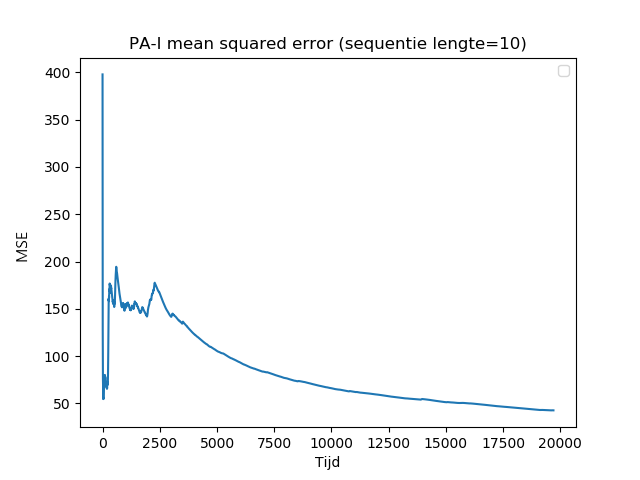
\includegraphics[width=\linewidth]{images/evaluatie/seqlen10.png}
\end{subfigure}
\begin{subfigure}{.49\textwidth}
  \centering
  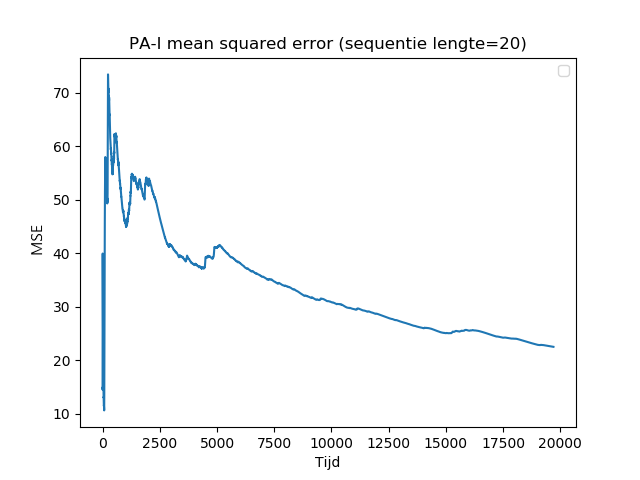
\includegraphics[width=\linewidth]{images/evaluatie/seqlen20.png}
\end{subfigure}
\begin{subfigure}{.49\textwidth}
  \centering
  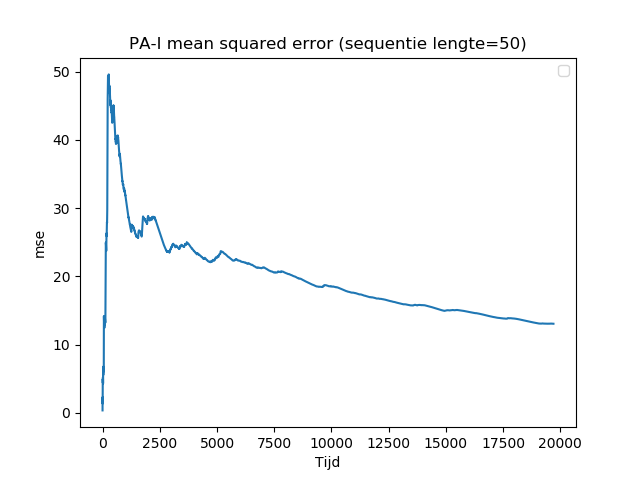
\includegraphics[width=\linewidth]{images/evaluatie/seqlen50.png} 
\end{subfigure}
\begin{subfigure}{.49\textwidth}
  \centering
  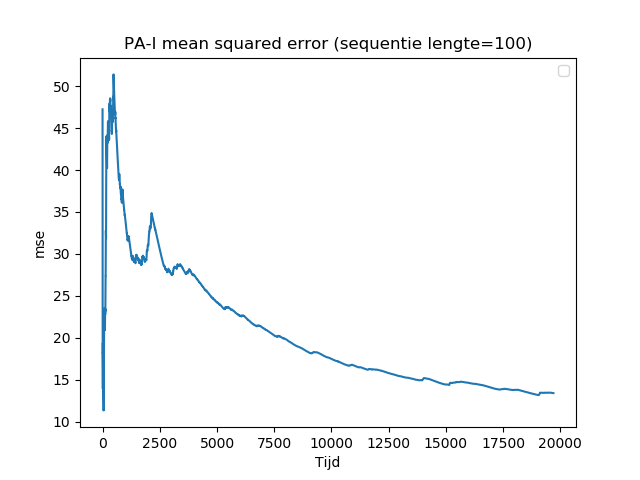
\includegraphics[width=\linewidth]{images/evaluatie/seqlen100.png}   
\end{subfigure}
\caption{De invloed van sequentielengte op de error}
\label{fig:seqlen error}
\end{figure}
\section{Algoritmes}
\subsection{Passive Aggressive Algorithm}
Er zijn enkele hyperparameters die ingesteld kunnen worden. $Max\_ iter$ is het maximum aantal iteraties dat het algoritme probeert bij te leren. Tol is een parameter die bepaalt of het algoritme vroegtijdig stopt. Dit gebeurt wanneer de fout na een leercyclus met minder dan tol verbetert. In de testomgeving, met $max\_ iter=25$ en $tol=0.1$, wordt deze vroegtijdige stop altijd behaald. Met andere woorden, na 25 iteraties heeft het algoritme de trainingsdata geleerd.
\\\\
Een laatste interessante parameter is C: de agressiviteit parameter. Hoe hoger deze is, hoe agressiever het algoritme de gewichten gaat bijwerken. De onderstaande figuren tonen de MSE van PA-I (links) en PA-II (rechts). C is de enige parameter die aangepast wordt.
\\\\
Bijna alle tests convergeren naar een MSE tussen tien en vijftien, met een gemiddelde tussen dertien en veertien. Wat het verschil is tussen PA-I en PA-II valt niet duidelijk te onderscheiden. In de paper van Crammer et al. \cite{pa algorithm} worden beide versies vergeleken op basis van instance noise en label noise. In beide gevallen scoren PA-I en PA-II aanzienlijk beter dan het standaardalgoritme. In dit experiment scoren PA-I en PA-II gelijkaardig.
\\\\
Figuur \ref{fig:gemiddeld aantal keer trainen pa} toont de invloed van C op het aantal keer trainen. Het verschil tussen de verschillende settings is klein. De “stappen” die genomen worden tijdens het trainen, zullen dus vaak klein genoeg zijn zodat C=1 agressief genoeg is. Het is dus niet nodig om hoge C-waarden (5-10) te gebruiken. Deze data is genomen over tien sessies, van elk 20000 iteraties, en duurde telkens gemiddeld 90 seconden. 
\\\\
\begin{figure}[h]
	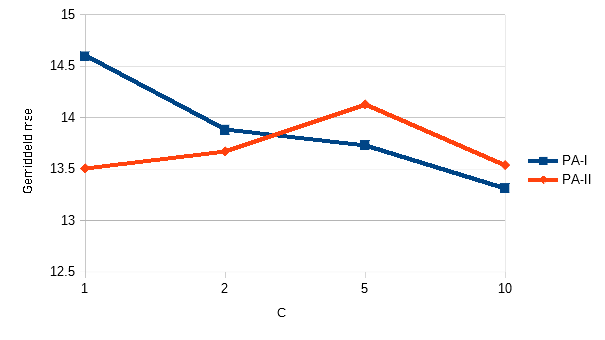
\includegraphics[width=\linewidth]{images/evaluatie/gemiddeldmsepa.png}
	\caption{De invloed van C op MSE van PA}
	\label{fig:invloed C op PA}
\end{figure}
\newpage
\begin{figure}[t]
	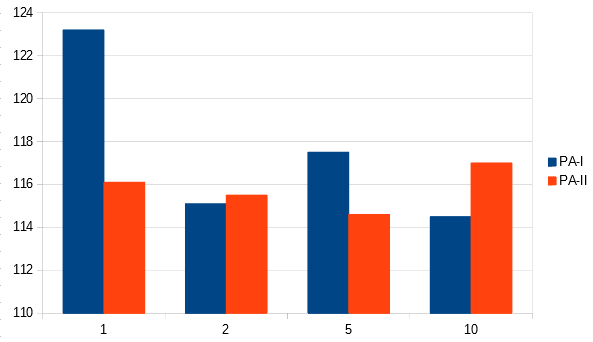
\includegraphics[width=\linewidth]{images/evaluatie/aantalkeertrainenpa.png}
	\caption{Gemiddeld aantal keer trainen PA}
	\label{fig:gemiddeld aantal keer trainen pa}
\end{figure}
\subsection{Decision Tree en Random Forest}
De belangrijkste parameter bij deze rule-based learners is de $max\_ depth$. Dit is een moeilijk in te schatten parameter, vooral voor de DT. Diepere DT’s maken betere voorspellingen, maar op een bepaald punt begint de DT te overfitten. Bij RF kan ook het aantal bomen ingesteld worden. Hoe meer bomen er gebruikt worden, hoe minder invloed ruis heeft op voorspellingen en hoe beter de voorspellingen worden.
\\\\
DT’s en RF’s convergeren beide naar ongeveer dezelfde MSE. Diepere bomen leiden evident naar een lagere MSE. Algemeen zijn grotere RF’s beter, maar in deze situatie is het verschil klein.
\\\\
Voor DT, daalt het gemiddeld aantal trainingen spectaculair tussen diepte drie en vier (figuur \ref{fig:invloed diepte en aantal bomen trainen}). Een DT van diepte drie zal dus geen goede oplossing zijn. RF’s daarentegen presteren wel goed met een diepte van drie. Een DT/RF dieper dan vier is niet nodig, aangezien dit geen groot voordeel oplevert en mogelijk overfit.
\\\\
De uitvoeringstijd (figuur \ref{fig:invloed diepte en aantal bomen uitvoeringstijd}) lijkt geen probleem te vormen voor grotere RF. Het verschil tussen de uitvoeringstijden van een RF met diepte drie en de anderen is te wijten aan het aantal keer dat getraind moest worden op diepte drie.

\begin{figure}[htp!]
\centering
\begin{subfigure}{\textwidth}
  \centering
    \hspace*{-0.75cm}                                                           
  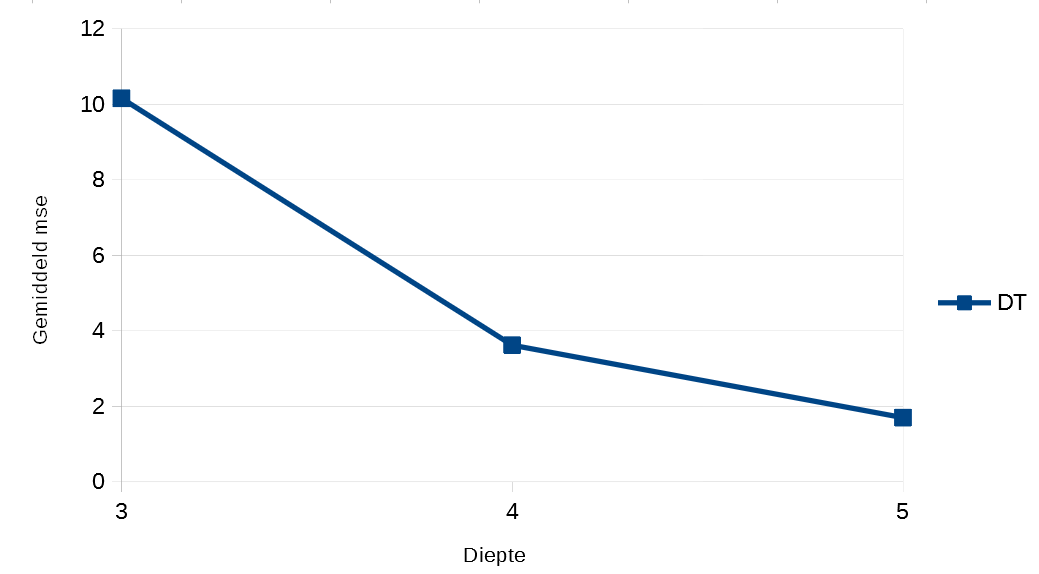
\includegraphics[width=\linewidth]{images/evaluatie/gemiddeldmsedt.png}
\end{subfigure}
\begin{subfigure}{\textwidth}
  \centering
  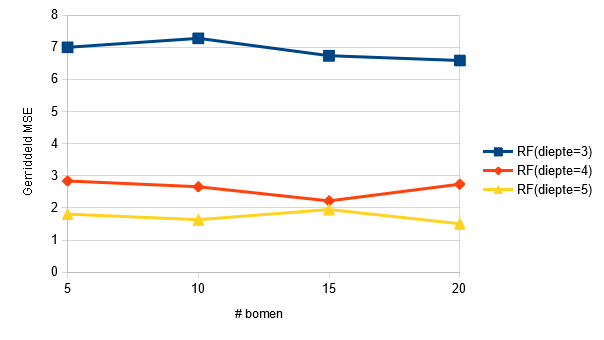
\includegraphics[width=\linewidth]{images/evaluatie/gemiddeldmserf.png}
\end{subfigure}
\caption{De invloed van diepte en aantal bomen op de gemiddelde MSE van DT en RF}
\label{fig:invloed diepte en aantal bomen mse}
\end{figure}
\begin{figure}[htp!]
\centering
\begin{subfigure}{\textwidth}
  \centering
    \hspace*{-0.75cm}                                                           
  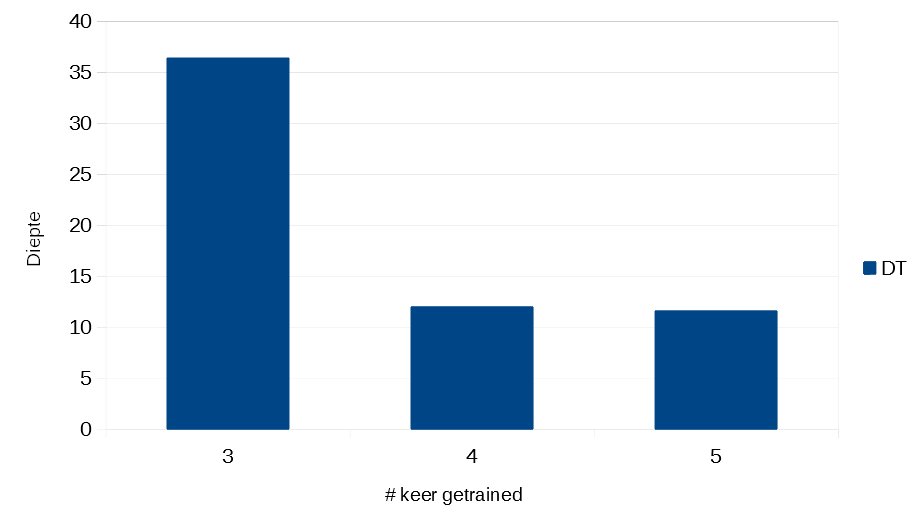
\includegraphics[width=\linewidth]{images/evaluatie/aantalkeertrainendt.png}
\end{subfigure}
\begin{subfigure}{\textwidth}
  \centering
  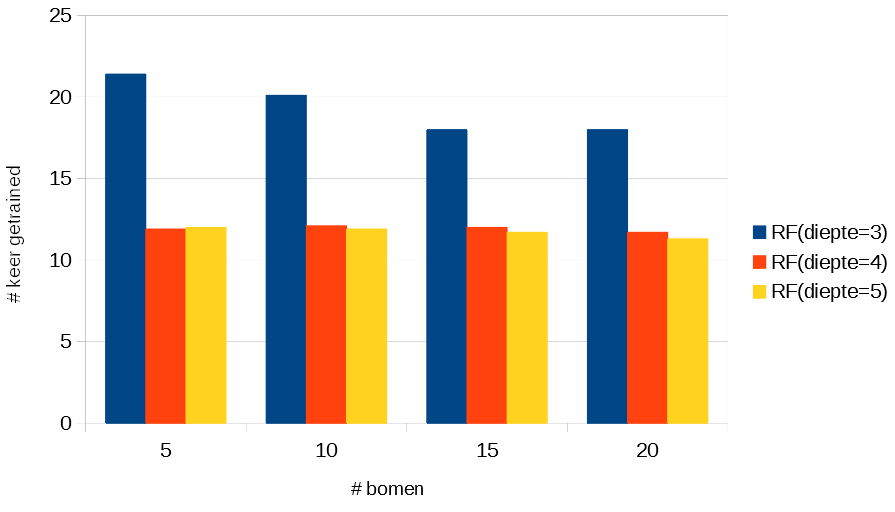
\includegraphics[width=\linewidth]{images/evaluatie/aantalkeertrainenrf.png}
\end{subfigure}
\caption{De invloed van diepte en aantal bomen op het gemiddeld aantal keer trainen van DT en RF}
\label{fig:invloed diepte en aantal bomen trainen}
\end{figure}
\begin{figure}[htp!]
\centering
\begin{subfigure}{\textwidth}
  \centering
  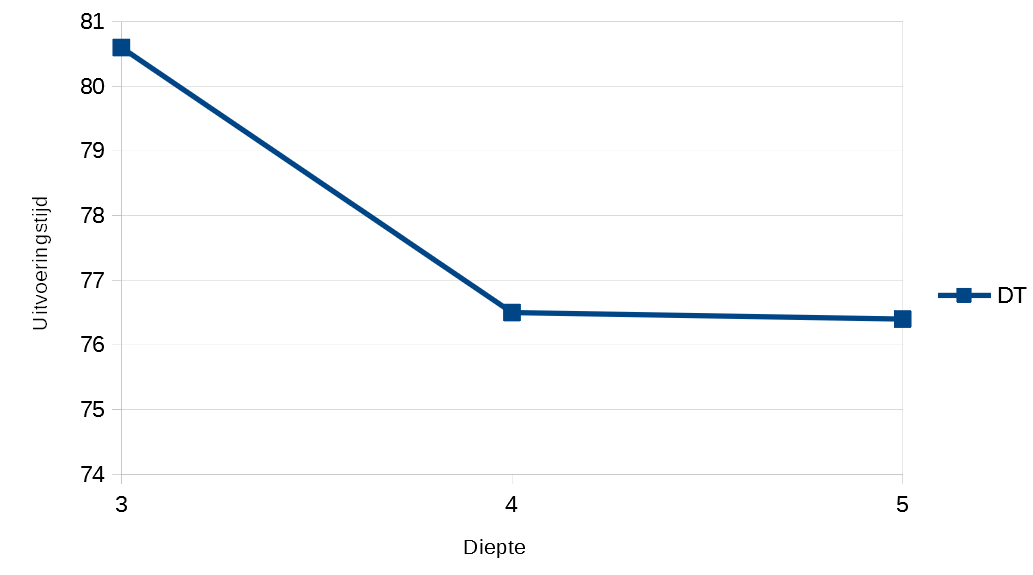
\includegraphics[width=\linewidth]{images/evaluatie/uitvoeringstijddt.png}
\end{subfigure}
\begin{subfigure}{\textwidth}
  \centering
  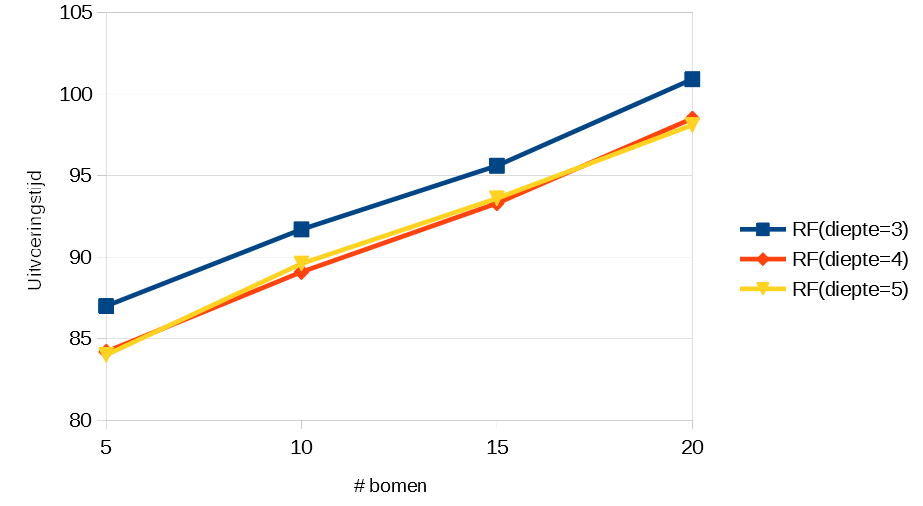
\includegraphics[width=\linewidth]{images/evaluatie/uitvoeringstijdrf.png}
\end{subfigure}
\caption{De invloed van diepte en aantal bomen op de uitvoeringstijd van DT en RF}
\label{fig:invloed diepte en aantal bomen uitvoeringstijd}
\end{figure}
\newpage
\section{Stochastisch bijleren}
In de onderstaande tabellen (tabellen \ref{tab:resultaten stochastisch bijleren PA}-\ref{tab:resultaten stochastisch bijleren RF}) zijn de resultaten te zien van gelijkaardige tests zoals in deel 2 van dit hoofdstuk. Het enige verschil met de voorgaande test, is de update-strategie voor het updaten van de verschillende modellen.
\\\\
In vorig hoofdstuk (sectie 2.10.1) werden verwachtingen opgesteld rond deze tests. Er werd verwacht dat de modellen deze probabilistische update-strategie aankunnen. In sommige gevallen is de MSE gelijkaardig aan de resultaten van de tests in deel 2 van dit hoofdstuk (PA-I, PA-II en RF en DT met diepte drie). Alle andere gevallen vertonen een betere MSE dan de originele tests. Dit komt waarschijnlijk door de hoeveelheid trainingsdata die gebruikt wordt. De probabilistische update-strategie zorgt ervoor dat er meer wordt bijgeleerd, waardoor er meer data beschikbaar is. De verwachting dat de modellen stochastisch kunnen bijleren is dus deels correct. Bomen van diepte drie moeten echter veel meer leren (aangezien $\Delta_c$ hoger is). Deze keer valt er wel een verschil te zien tussen een klein RF en een groot RF. Een groter RF traint minder vaak.
\\\\
Bij DT en RF is de stijging van het gemiddeld aantal keer trainen het grootst. PA presteerde al slechter dan de andere modellen waardoor de stijging hier minder extreem is. De algemene stijging is te wijten aan het feit dat er geen tolerantiegrens meer is. Het verschil tussen de voorspelde cadans en het fietsersmodel ($\Delta_c$) kan maar enkele rpm groot zijn, het kan nog steeds een update veroorzaken. Figuur \ref{fig:stochastic diff rf} toont hoe $\Delta_c$ evolueert doorheen de test voor een RF bestaande uit 20 bomen met diepte vier. Dit model update gemiddeld 59.6 keer. Aan de grafiek te zien zijn deze updates meestal doorgevoerd wanneer het verschil klein is ($\Delta_c<2$).
 

\begin{table}[hp!]
\centering
\begin{tabular}{|l|l|l|l|l|l|}
\hline
\multicolumn{2}{|l|}{\multirow{2}{*}{Passive Aggressive Algorithm}}                               & \multicolumn{4}{c|}{c}                                        \\ \cline{3-6} 
\multicolumn{2}{|l|}{}                                                                            & 1             & 2             & 5             & 10            \\ \hline
\multirow{2}{*}{Gemiddelde MSE}                                                           & PA-I  & 14.76 (+1\%)  & 14.63 (+5\%)  & 14.66 (+7\%)  & 14.60 (+10\%) \\ \cline{2-6} 
                                                                                          & PA-II & 14.52 (+7\%)  & 14.50 (+6\%)  & 14.05 (-1\%)  & 15.56 (+15\%) \\ \hline
\multirow{2}{*}{\begin{tabular}[c]{@{}l@{}}Gemiddeld aantal \\ keer trainen\end{tabular}} & PA-I  & 175.6 (+42\%) & 170.3 (+48\%) & 148.8 (+26\%) & 147.7 (+28\%) \\ \cline{2-6} 
                                                                                          & PA-II & 170.3 (+46\%) & 168.1 (+45\%) & 176.0 (+53\%) & 179.0 (+54\%) \\ \hline
\end{tabular}
\caption{Resultaten stochastisch bijleren PA}
\label{tab:resultaten stochastisch bijleren PA}
\end{table}

\begin{table}[hp!]
\begin{tabular}{|l|l|l|l|}
\hline
\multirow{2}{*}{Decision tree}                                           & \multicolumn{3}{c|}{Diepte}                    \\ \cline{2-4} 
                                                                         & 3              & 4             & 5             \\ \hline
Gemiddelde MSE                                                           & 9.37\phantom{1} (-8\%)    & 2.41 (-33\%)  & 1.06 (-37\%)  \\ \hline
\begin{tabular}[c]{@{}l@{}}Gemiddeld aantal \\ keer trainen\end{tabular} & 160.8 (+341\%) & 88.9 (+640\%) & 51.3 (+342\%) \\ \hline
\end{tabular}
\caption{Resultaten stochastisch bijleren decision tree}
\label{tab:resultaten stochastisch bijleren DT}
\end{table}

\begin{table}[htp!]
\centering
\begin{tabular}{|l|l|l|l|l|l|}
\hline
\multicolumn{2}{|l|}{\multirow{2}{*}{Random forest}}                                                 & \multicolumn{4}{c|}{Aantal bomen}                                 \\ \cline{3-6} 
\multicolumn{2}{|l|}{}                                                                               & 5              & 10             & 15             & 20             \\ \hline
\multirow{3}{*}{Gemiddelde MSE}                                                           & Diepte 3 & 7.35 (+5\%)    & 7.42 (+2\%)    & 7.33 (+9\%)    & 7.37 (+12\%)   \\ \cline{2-6} 
                                                                                          & Diepte 4 & 1.47 (-48\%)   & 1.38 (-38\%)   & 1.37 (-38\%)   & 1.35 (-50\%)   \\ \cline{2-6} 
                                                                                          & Diepte 5 & 0.56 (-69\%)   & 0.59 (-64\%)   & 0.53 (-73\%)   & 0.56 (-63\%)   \\ \hline
\multirow{3}{*}{\begin{tabular}[c]{@{}l@{}}Gemiddeld \\ aantal keer \\ trainen\end{tabular}} & Diepte 3 & 145.3 (+578\%) & 143.8 (+615\%) & 145.4 (+707\%) & 144.7 (+704\%) \\ \cline{2-6} 
                                                                                          & Diepte 4 & 72.8\phantom{1} (+511\%)  & 58.2\phantom{1} (+380\%)  & 61.6\phantom{1} (+413\%)  & 59.6\phantom{1} (+409\%)  \\ \cline{2-6} 
                                                                                          & Diepte 5 & 40.4\phantom{1} (+236\%)  & 31.8\phantom{1} (+167\%)  & 33.4\phantom{1} (+185\%)  & 30.4\phantom{1} (+169\%)  \\ \hline
\end{tabular}
\caption{Resultaten stochastisch bijleren random forest}
\label{tab:resultaten stochastisch bijleren RF}
\end{table}




\begin{figure}[hp]
	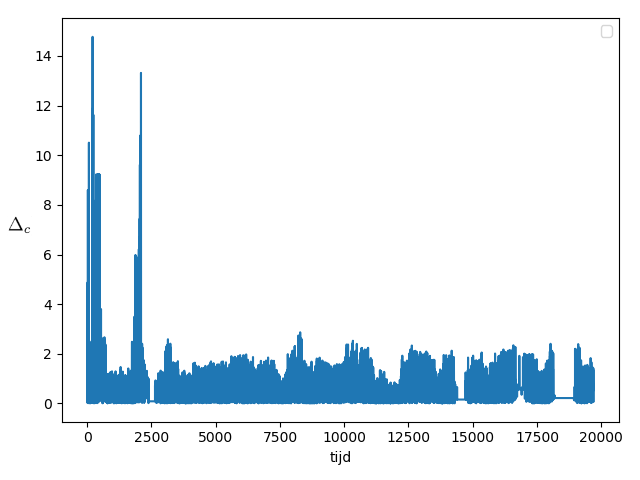
\includegraphics[width=\linewidth]{images/evaluatie/stochastic_diff_rf.png}
	\caption{Het absoluut verschil tussen het fietsersmodel en de voorspellingen ($\Delta_c$) in verloop van tijd}
	\label{fig:stochastic diff rf}
\end{figure}
\newpage
\section{Conceptuele drift}
Wederom wordt dezelfde test als in deel 2 van dit hoofdstuk gebruikt als basis om resultaten te verkrijgen van de twee algoritmes die omgaan met conceptuele drift. Het model voor deze test is een RF bestaande uit 20 bomen met diepte vier. Eerst wordt het RF getraind op basis van een fietsersmodel in functie van het DC-koppel (gemiddeld koppel) voor 20000 iteraties. Vervolgens “stopt” de fiets en wordt het fietsersmodel vervangen door een ander model, dit keer in functie van de helling. In werkelijkheid wordt een nieuw fietsobject geïnstantieerd en maakt dit gebruik van de bestaande cadans controller. Deze nieuwe actor fietst dan voor 40000 iteraties. De tweede fietstocht is langer genomen om na te gaan of de datastructuren wel groot genoeg zijn, zodat het hele concept in deze structuur past. Er worden vier verschillende groottes (500, 750, 1000 en 1250) met elkaar vergeleken die respectievelijk overeenkomen met data voor 10, 15, 20 en 25 trainingen. Deze worden dan vergeleken met een referentietest, een uitvoering zonder drift technieken. 
\\\\
In figuur \ref{fig:conceptuele drift vergelijking} is te zien dat wanneer er minder data wordt bijgehouden, er in totaal minder moet geleerd worden. Dit verschilt met de verwachting, die opgesteld is in sectie 2.11.4, dat kleinere structuren slechter zouden presteren dan grotere structuren. Waarschijnlijk is het betere resultaat juist te wijten aan de kleine structuur, waardoor er snel vergeten wordt. In grotere structuren blijft data langer rondhangen. Het oude concept vult niet de hele structuur. Hierdoor zal er meerdere keren geüpdatet moeten worden vooraleer het nieuwe concept geleerd is, net zoals wanneer er geen drift mechanisme is. Uiteindelijk is het oude concept vergeten, maar hiervoor was er veel meer data nodig. Bijvoorbeeld, bij het veranderen van concept hebben we twee of drie keer zoveel data nodig van situatie A, die ook voorkomt tijdens de vorige fietstocht (situatie is hier de algemene toestand van de fiets). Vervolgens komt situatie B die weeral twee of drie keer zoveel data nodig heeft, omdat het sliding window nog niet genoeg vergeten heeft. Uiteindelijk hebben we zoveel data toegevoegd van het nieuwe concept dat het oude concept helemaal vergeten is. Maar omdat er zoveel meer data nodig was, zijn nog niet alle situaties bekeken. Als de fiets dan in een ongeziene situatie komt, kan data van situatie A al vergeten worden. Stel dat situatie A uiteindelijk terugkomt, dan moet dit opnieuw geleerd worden. Deze keer minder aangezien er geen conflict is met een ouder concept. Dit probleem is zichtbaarder in een sliding window dan bij sampling, aangezien sampling "sneller" data vergeet. Elke keer er een observatie toegevoegd wordt, is er een kans dat er één verwijderd wordt. Waardoor elke situatie in mindere mate aanwezig is, maar toch nog genoeg om een goede voorspelling te leveren. Merk op dat voor zowel sliding window als sampling bij grootte 500 er minstens 1750 observaties bekeken zijn om met conceptuele drift om te gaan.

\begin{figure}[th]
	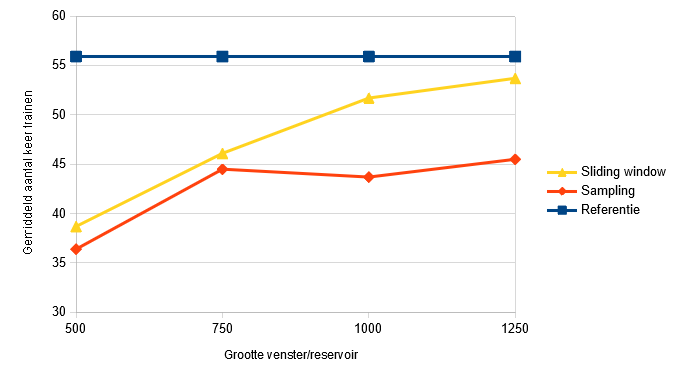
\includegraphics[width=\linewidth]{images/evaluatie/conceptuele_drift_vergelijking.png}
	\caption{Resultaten van beide technieken om met conceptuele drift om te gaan.}
	\label{fig:conceptuele drift vergelijking}
\end{figure}


\chapter{Discussie}
\section{Algoritmes}
Het vorige hoofdstuk toont de resultaten van de verschillende algoritmes. RF en DT presteren duidelijk beter dan beide types van PA. DT presteert goed, maar is nog steeds bekend om het slecht omgaan met ruis en het overfitten. Aangezien het verschil in uitvoeringstijd tussen DT en RF minimaal is, is het altijd beter om een RF te gebruiken. Alhoewel in de test blijkt dat de grootte van het RF geen al te grote impact heeft op de uitvoeringstijd, kan dit mogelijk nog een probleem vormen door de beperkte rekenkracht van de Raspberry Pi. Het controleprogramma voor de fiets zal immers parallel lopen met de cadanscontroller. Gelukkig heeft de Raspberry Pi vier cores en is een RF makkelijk te parallelliseren (door het instellen van het aantal parallelle taken).
\\\\
Voor een RF zijn volgende hyperparameters aangeraden:
\begin{gather*}
\text{RF \tab diepte=4 of 5, aantal bomen=10-20}
\end{gather*}
Een groot nadeel van RF is dat het niet goed om kan met ongeziene omstandigheden. Bijvoorbeeld als het algoritme van niets of weinig data begint, kan het niet uit de reeds geziene data een goede voorspelling maken (t.o.v. lineaire regressie voor een simpel lineair probleem).
\section{Waarheid}
In de verschillende testen werd het fietsersmodel altijd als waarheid (\textit{ground truth}) gezien. Dit kan echter niet gebruikt worden aangezien dit ongekend is. Als de fietser een update wilt doen, dan weet het algoritme niet hoe hard het algoritme moet aanpassen. Als de fietser sneller wilt trappen, is het dan twee rpm sneller of vijf? Dit is in deze thesis niet onderzocht, maar vormt nog een potentieel probleem in het succes van de real-time cadansaanpassing in een automatische fiets transmissie.
\\\\
Het voornaamste probleem dat zich hier voordoet, is dat twee achtereenvolgende trainingen data zullen genereren die in conflict gaan met elkaar. Stel dat de fietser 60 rpm trapt. De eerste keer dat hij op de knop duwt, wordt er trainingsdata gegenreerd met als doelvariabele 65 rpm. De tweede keer wordt er gelijkaardige data gegenereerd, maar dan met een doelvariabele van 70 rpm. Een mogelijke oplossing voor dit probleem, is het kijken naar de dichtst bijzijnde buren in de trainingsset en de doelvariabelen te updaten volgens de afstand. Hoeveel de doelvariabele bijgewerkt moet worden, zou exponentieel moeten dalen voor observaties die ver weg liggen.
\section{Conceptuele drift}
In sectie 3.4 werden de resultaten van twee algoritmes, statisch schuivend venster en bevoordeelde reservoir sampling, getoond. In beide gevallen moest er minstens drie keer zoveel geleerd worden om het nieuwe concept te leren, wat toch wel een groot verschil is met het beginnen vanaf nul. Deze technieken doen het alleszins wel beter dan geen “vergeet” algoritme. Het voornaamste probleem hier is dat mensen die deze fiets tweedehands kopen of als leen-, familiefiets gebruiken, een slechtere ervaring zullen hebben dan mensen die de fiets nieuw kopen en enkel zelf gebruiken.
\section{Verder werk}
De huidige implementatie van een RF, geïmplementeerd in de \texttt{scikit-learn} bibliotheek, doet niet aan lokale regressie in de bladeren. In plaats daarvan bevatten de bladeren een gewoon getal. Mogelijk kan lokale regressie in de bladeren een betere prestatie leveren.
\\\\
Er werd een probleem aangehaald met een RF: het kan niet goed om met ongeziene omstandigheden, zoals wanneer de fiets nog niet is ingesteld door de gebruiker. Er wordt hiervoor volgende oplossingen voorgesteld: 

\begin{itemize}
\item een standaard model voorzien
\item hetgeen wat het RF voorspelt veranderen van de eigenlijke cadans naar een verschil ten opzichte van een ingestelde basis cadans.
\end{itemize}

\noindent Een standaard model voorzien vergt extra werk. Het tweede voorstel daarentegen is makkelijk te implementeren. Trappen op een basis cadans is gelijkaardig met hoe de fiets werkt zonder cadanscontroller (mits er niet op de knoppen geduwt wordt).
\\\\
Voor het deel van conceptuele drift, zou de grootte van het venster of reservoir bepaald kunnen worden aan de hand van gebruikerstesten. Daarnaast is het uitwerken van een profielensysteem ook zeker een interessant topic om verder aan te werken. Een profielensysteem houdt verschillende modellen bij van verschillende personen. Indien iemand gaat fietsen, met een reeds bestaand profiel, zou het profielensysteem het overeenkomstige profiel moeten activeren.


\chapter{Conclusie}
Eerst werd er een realistische geparametriseerde simulatie opgezet. Die houdt rekening met verschillende lasten, maar niet allemaal. De simulatie zorgt ervoor dat er gemakkelijk en snel data kan gegenereerd worden voor verschillende tests. Ten tweede werden enkele algoritmes besproken en geëvalueerd. De resultaten tonen dat PA niet geschikt is voor dit probleem, aangezien de fout te groot is en dat PA te vaak moet bijleren. DT en RF presteerden hier goed. Ten derde werd nagegaan of de algoritmes kunnen omgaan met een stochastische update-strategie. Wederom presteert PA slecht. Binaire beslissingsbomen, zowel bij DT als RF, met diepte drie presteren hier ook slecht omdat het verschil tussen fietsersmodel en voorspelling vrij groot blijft gedurende de test. Uit deze twee tests werd er besloten dat enkel DT en RF, met diepte vier of dieper, geschikt zijn voor dit probleem. Uiteindelijk werd de keuze gemaakt om enkel verder te werken met een RF. Er werd wel nog een probleem aangehaald met een RF: het kan niet goed om met ongeziene omstandigheden, zoals wanneer de fiets nog niet is ingesteld door de gebruiker. Er wordt hiervoor volgende oplossingen voorgesteld: 

\begin{itemize}
\item een standaard model voorzien
\item hetgeen wat het RF voorspelt veranderen van de eigenlijke cadans naar een verschil ten opzichte van een ingestelde basis cadans.
\end{itemize}

\noindent Vervolgens werden twee technieken getest die kunnen omgaan met conceptuele drift, het veranderen van concept over tijd. De drift die hier getest werd was abrupt in deze context. De resultaten tonen aan dat kleinere structuren beter presteren dan grotere. Sampling presteert in het algemeen beter dan een sliding window. Of omgaan met conceptuele drift noodzakelijk is, hangt af van hoe men de fiets gebruikt. Er werd ten slotte nog een probleem aangehaald met de tests en trainingsdata. In de simulatie werd een “waarheid” (\textit{ground truth}) berekend met behulp van het fietsersmodel. In realiteit bestaat dit niet en zullen updates incrementeel moeten doorgevoerd worden. Dit moet zeker nog uitgewerkt worden. Uiteindelijk moet er ook nog een implementatie voorzien worden die samenwerkt met de fietscontroller van Ellio.
\\\\
Of een RF het meest geschikte algoritme is, is moeilijk te zeggen. Er zijn zoveel verschillende algoritmes van machinaal leren dat het praktisch onmogelijk is om ze allemaal te bekijken. Een type algoritme dat hier niet aangehaald is, maar mogelijk wel nog goed kan presteren in clustering.
\\\\
De cadanscontroller moet natuurlijk ook nog uitgewerkt worden, zodat het samenwerkt met de fietscontroller.
\chapter*{Appendix}
\addcontentsline{toc}{chapter}{Appendix}
\section*{IntuEdrive}
\addcontentsline{toc}{section}{IntuEdrive}
Ir. Tomas Keppens werkte als departementshoofd bij Toyota toen hij in 2010 met het IntuEdrive project begon. In het kader van aan aantal masterproeven aan de KU Leuven werd het project stap per stap uitgewerkt.. In het academiejaar 2016-2017 werkte ingenieursstudent Jorrit Heidbuchel de aansturing van het intuEdrive CVT systeem uit. Halverwege 2017 was er het eerste prototype. Later dat jaar richtten Tomas Keppens en Jorrit Heidbuchel samen intuEdrive op.
\\\\
IntuEdrive wil mobiliteit duurzamer en efficiënter maken door twee-wielmobiliteit veiliger te maken. Het bedrijf bouwt en ontwikkelt E-bikes die perfect passen in het leven van zijn klanten: makkelijk in gebruik, veilig en betrouwbaar.
\\
Vandaag telt IntuEdrive 4 werknemers. CoSaR gaat in het najaar van 2019 voor het eerst in productie en mikt in 2020 op een verkoop van 1000 stuks in België.
\begin{figure}[h]
  \centering
  
\includegraphics[width=0.5\linewidth]{images/logo_intuedrive.png}
  \caption{Logo IntuEdrive}
  \label{fig:Logo IntuEdrive}
\end{figure}
\newpage
\begin{thebibliography}{9}
\addcontentsline{toc}{section}{Bibliografie}
\bibitem{hardware implementation} 
Heidbuchel, J. (2017); Hardware Implementation and Control Strategy of a High Dynamic CVT Transmission for an E-Bike; KULEUVEN
 
\bibitem{randomforest paper} 
Breiman, L. (2001); Random Forests; UC BERKELEY

\bibitem{encoding cyclical features} 
London I. (2016); Encoding cyclical continuous features - 24-hour time; https://ianlondon.github.io/blog/encoding-cyclical-features-24hour-time/

\bibitem{preprocessing faq}
Sarle, W. comp.ai.neural-nets FAQ; http://www.faqs.org/faqs/ai-faq/neural-nets/part1/preamble.html

\bibitem{pa algorithm}
Crammer, Dekel, Keshet, Shalev-Shwartyz, Singer (2006); Online Passive-Aggressive Algorithms; Hebrew University of Jerusalem

\bibitem{cvt wikipedia}
https://en.wikipedia.org/wiki/Continuously\_ variable\_ transmission

\bibitem{vermogen wikipedia}
https://nl.wikipedia.org/wiki/Vermogen\_\%28natuurkunde\%29

\bibitem{random forest wikipedia}
https://en.wikipedia.org/wiki/Random\_ forest

\end{thebibliography}






\newpage
% ----------------------- Achterblad ------------------------------
% Vergeet niet de tekst aan te passen:
% - Afdeling
% - Adres van de afdeling
% - Telefoon en faxnummer
% -----------------------------------------------------------------
\thispagestyle{empty}
\sffamily
%
\begin{textblock}{191}(113,-11)
{\color{blueline}\rule{160pt}{5.5pt}}
\end{textblock}
%
\begin{textblock}{191}(168,-11)
{\color{blueline}\rule{5.5pt}{59pt}}
\end{textblock}
%
\begin{textblock}{183}(-24,-11)
\textblockcolour{}
\flushright
\fontsize{7}{7.5}\selectfont
\textbf{Computerwetenschappen}\\
Celestijnenlaan 200 A bus 2402\\
3000 LEUVEN, BELGI\"{E}\\
tel. + 32 16 32 77 00\\
fax + 32 16 32 79 96\\
www.kuleuven.be\\
\end{textblock}
%
\begin{textblock}{191}(154,-7)
\textblockcolour{}
\includegraphics*[height=16.5truemm]{sedes}
\end{textblock}
%
\begin{textblock}{191}(-20,235)
{\color{bluetitle}\rule{544pt}{55pt}}
\end{textblock}
\end{document}
